\begin{savequote}[75mm]
Isn't it a pleasure to study and practice what you have learned?  Isn't it also great when friends visit from distant places?
\qauthor{First words of the Analects of Confucious}
\end{savequote}

\chapter{A Search and Learning Model of Export Dynamics}
\hfill{} \emph{with Jonathan Eaton, C.J. Krizan, and James R. Tybout}

\newthought{Research on exporting} has been digging deeper into microeconomics data to
understand the barriers that producers face in entering foreign markets and
their implications for export dynamics. Firm-level datasets have provided
insights first into the costs of exporting at all, and then, as data became
available, to penetrating individual markets. We take this analysis one step
forward by examining exporters' relationships with individual buyers in a
market, both descriptively and through the lens of a dynamic model.

\subsection{Scope}

We begin by summarizing patterns in a decade's worth of data on individual
merchandise shipments from Colombia to the United States. First, following
work by some of the authors (Eaton et al., 2008), we review patterns of
entry into the U.S. market of individual Colombian exporters across
different cohorts. We note that most new exporters drop out of the U.S.
market within a year, but those who survive this shakedown period have much
lower exit rates in the future. Indeed, surviving members of new cohorts
tend to expand their sales very rapidly, causing their market shares to grow
as they mature. After a decade, nearly a quarter of total Colombian exports
to the U.S. originate from firms that were not supplying the U.S. market at
the beginning of the period.

We then look at relationships between buyers and sellers. Colombian firms
which export to the U.S. ship at least once per year to an average of 1.3
U.S. clients. In contrast, U.S. firms place at least one order per year with
an average of 2.2 Colombian suppliers if they deal with Colombian firms at
all. Overall, the distribution of U.S. clients across Colombian exporters is
very nearly Pareto, with a handful of large sellers accounting for a
substantial fraction of total shipments. Most buyer-seller matches are
short-lived, lasting less than two years, on average. Matches are even less
durable if they begin with a small initial shipment. But enough exporters
gain buyers each period that the ergodic distribution implied by the
transitions and by entry replicates closely the distribution in the cross
section.

Finally, we develop a model that is consistent with these facts. It is based
on the conjecture that firms' exporting behavior reflects search and
learning processes in a foreign market. That is, producers who are
interested in a particular market devote resources to identifying potential
buyers there. When they find one, they learn something (receive a noisy
signal) about the appeal of their products in this market. Taking stock of
the available information, these firms update their beliefs concerning the
scope for export profits, and they adjust the intensity of their search
efforts accordingly, seeking to maximize their expected profit streams. At
the same time, firms manage their portfolio of existing clients, investing
in their profitable business relationships and letting the others expire.
These features of the model are not only motivated by the exporting patterns
observed in the data, but also by the exporting strategies documented by a
series of interviews with Colombian exporters (Dom\'{\i}nguez et al, 2013).
Interviewed exporters described engaging in costly strategies both to search
for new clients and to maintain existing relationships alive. They also
frequently mentioned learning from previous relationships about the appeal
of their products in a particular market, and using that information to
adjust their searching behavior.

Fit to our data on shipments and business relationships, the model
quantifies the role of several frictions in shaping firm-level export
dynamics. We estimate that for non-exporters, the costs of maintaining
low-level searches for clients in the U.S. are small, amounting to \$1,405
per year for an expected yield of one potential client every two years.
However, search costs are very convex in buyer arrival hazards, rising to
\$51,471 for an expected yield of one potential client per year. Both of
these figures describe the search costs for a firm that has not yet
established a successful business relationship abroad. But network effect
are very important. We estimate that after the first relationship is formed,
search costs for one client every two years drop to \$106, and \$3,898 for
one client per year. Finally, once a successful match is formed, we estimate
that it costs exporters \$2,855 dollars per shipment to maintain the
relationship. As a benchmark, the Doing Business project of the World Bank
estimates that procedures required to export a one-container shipment cost
\$1,745 in Colombia in 2005. Even when a seller pays the fixed cost, her
relationship dissolves with probability 0.27 per year for exogenous reasons.

In addition to trade costs, the model quantifies the effects of learning on
exporter behavior. We estimate that on average, only 1 in 5 potential buyers
that an exporter meets will be interested in forming a business
relationship. However, this success rate varies substantially across
sellers, so they adjust their search intensities dramatically as they form
opinions concerning the scope of the market for their particular product. A
typical firm which has met four potential buyers will choose a match hazard
of 1.35 (new clients per year) if all of its encounters have led to
successful business relationships, while it will choose a hazard of 0.22 if
each encounter has been a failure.

This learning process, in combination with the various trade costs mentioned
above, induces frictions and irreversibilities in export responses to
marketwide shocks. We conclude our analysis with some experiments that
quantify their implications for export dynamics. A 20 percent reduction in
the cost of searching for new clients leads to an increase in total exports
of around 5 percent, which takes some time to kick in. Increased exports are
mostly explained by the entry of new sellers into exporting, and to a lesser
extent by an increase in the mean number of clients per seller. In turn, a
decrease of 20 percent in the per-shipment fixed cost leads to a much more
marked increase in both the number of exporters and the mean number of
clients, and also to an increase in mean sales per client. The latter occurs
despite the entry into exporting of less productive sellers, and is
explained by increased search by the more productive firms.

\subsection{Relation to literature}

While we look at the evolution of firms' sales in a particular market, our
analysis is related to the literature on the dynamics of firm size in
general. The model explains the size distribution of firm sales through two
interacting mechanisms. One, as in Melitz (2003), Bernard et al. (2003),
Luttmer (2007), and Irarrazabal and Opromolla (2006), is firm efficiency:
More efficient firms sell more to a given set of buyers by having a lower
price or a higher quality product. A second is that some firms have larger
networks of buyers than others, as in Jackson and Rogers (2007) or Chaney
(2011).

Investments in building a client base constitute a type of sunk cost, so our
model also relates to the export hysteresis literature (Dixit, 1989; Baldwin
and Krugman, 1989; Das, et al., 2007; Alessandria and Choi, 2007;
Alessandria et al., 2010), where firms pay a one-shot start-up cost to break
into new markets. But unlike these formulations, our sunk costs are incurred
on the client margin rather than the country margin, and they pay off in
terms of market knowledge and reputation as well as revenue streams. These
features of our model allow us to explain why new exporters who don't exit
tend to rapidly expand, and why established exporters' sales are relatively
stable. They also explain why many firms export for short periods on a very
small scale.

Our formulation is also related to the two-period learning models developed
by Rauch and Watson (2003) and Albornoz et al (2012). In the former,
importers experiment with foreign suppliers by placing trial orders with
them, and they gain access to a supplier network if they establish a
successful business relationship. In the latter, firms choose to experiment
in markets with low entry costs in order to learn about their product's
appeal elsewhere. Like our model, these formulations provide interpretations
for the fact that when new exporters survive, their exports tend to grow
rapidly.\renewcommand{\baselinestretch}{1}\footnote{%
Ruhl and Willis (2008) also note this pattern in plant-level export data and
show that market entry costs are insufficient to explain it.}

Finally, in allowing firms to attract more buyers by incurring greater
costs, our analysis relates to Drozd and Nozal (2012) and Arkolakis (2009,
2010). By positing that firms face marketing costs that are convex in the
number of foreign clients they service, Arkolakis also accounts for
small-scale exporters and the age-dependence of export growth rates.
However, since all exporting relationships last a single period in his
models and learning is absent, Arkolakis's models\ do not explain the
irreversibilities observed in firms' exporting behavior, nor do they speak
to the duration of matches.

\section{Firm-Level Trade: Transaction Level Evidence}
\label{sec:data}

\subsection{Data}

The empirical motivation for our model comes from a comprehensive data set
that describes all imports by buyers in the United States from Colombian
exporters (as well as other origins ) during the period 1992-2009. The
source is the U.S. Census Bureau's Longitudinal Foreign Trade Transactions
Database (LFTTD). Each record includes a date, the US dollar value of the
product shipped, a 6-digit harmonized system product code, a quantity index,
and, critically, ID codes for both sellers and buyers. These IDs allow us to
identify the formation and dissolution of business relationships between
individual buyers in the U.S. and sellers in Colombia, hereafter referred to
as \textquotedblleft matches.\textquotedblright \footnote{%
There are two ways to track U.S. importers in the LFTTD: Employment
Identification Numbers (EINs) and the firm identifiers in the Longitudinal
Business Database ("alphas"). Though an EIN does not necessarily identify a
complete firm, it is unique to a firm, and there is one associated with
every import transaction. Alphas map to entire firms, but the match rate
between trade transactions and alphas is only about 80 percent (Bernard,
Redding, and Schott, 2009). To maximize the coverage of our sample, we use
Employment Identification Numbers (EIN) to identify U.S. buyers.\medskip}\ 

To identify foreign exporters, the U.S. import transactions records include
a manufacturer's identification code.\footnote{%
This variable is based on Block 13 of CBP form 7501, the import declaration
form and customs brokers are required to input the data.} This field is an
amalgamation of the manufacturer's country, company name, street address,
and city. Anecdotal information from customs brokers indicates that commonly
used software constructs it automatically as the name and address
information is entered in other fields. So this variable is sensitive to
differences in the way exporters' names and addresses are recorded as they
pass through customs, and shipments from the same exporter can appear to
originate from distinct Colombian firms. To gauge the importance of this
problem, we have conducted various checks on the matches that are based on
this variable; these are explained in the Appendix.

We limit our analysis to transactions between non-affiliated trade partners,
and we consider only imports of manufactured goods. The latter restriction
notably excludes oil and coffee exports, which constitute the bulk of trade
between the two countries and are dominated by a few Colombian sellers.%
\footnote{%
Colombian commercialization of coffee is centralized to an important degree
by the National Federation of Coffee Growers. A few players also dominate
oil exports.} Our final data set of manufacturing transactions spans the
years 1992-2009. It contains 26,625 unique Colombian exporters, 12,921
unique U.S. importers, and 42,767 unique trading pairs. Value data have been
deflated to 1992 prices using the U.S. CPI. Since we exclude a number of
large HS codes from our data, as well as affiliated trade, and because we
also lose information due to disclosure restrictions, the total value
covered by our data is not comparable to total Colombian exports to the U.S.
Table \ref{tab:ap_dat_comp} in Appendix \ref{sec:data_check} compares
patterns in our sample to patterns in official aggregates from both the U.S.
and Colombia.

In addition to U.S. customs records, we use establishment level survey data
from Colombia's national statistics agency (Departmento Administrativo
Nacional de Estadistica, or DANE). These data provide annual information on
the sales volumes, exports, and other characteristics of all Colombian
manufacturing plants with at least 10 workers. Because they have been widely
analyzed, we do not discuss summary statistics for this data set herein.
Later, however, when estimating our search and learning model, we use such
statistics to characterize the size distribution of Colombian firms, the
fraction of Colombian plants that export and, among these firms, the
relationship between exports and domestic sales.

\subsection{Exports and exporters}


Following Brooks (2006) and Eaton et al. (2008), Tables \ref%
{tab:firm_num_by_cohort}-\ref{tab:exp_per_firm_by_cohort} provide various
annual measures of Colombian exports of manufactured goods to the United
States for the years 1992-2009.\footnote{%
Similar tables for Colombian exports of all goods and to all destinations
appear in Eaton, et al, 2008.\medskip \medskip} Each column follows an
exporting cohort---i.e., a group of firms that began exporting in a
particular year---from the year of its appearance through time. The tables
report number of exporters, total exports, and exports per firm,
respectively. Note that, since we don't know the history of firms before
1992, the 1992 \textquotedblleft cohort\textquotedblright\ consists of all
firms present that year, regardless of when they began exporting; given
re-entry. This implies that the first few cohorts are in general
overestimated in terms of their initial size. Nonetheless, the patterns
highlighted below apply also to the most recent cohorts. \bigskip

\begin{sidewaystable}[bph]
\centering
{\footnotesize
    \begin{tabular}{l|rrrrrrrrrrrrrrrrrr|r} \hline \hline \\
year & 1992  & 1993  & 1994  & 1995 & 1996 & 1997 & 1998 & 1999  & 2000  & 2001  & 2002  & 2003  & 2004  & 2005  & 2006  & 2007  & 2008  & 2009  & total\\\hline\\
1992 & 2,232 &       &       &      &      &      &      &       &       &       &       &       &       &       &       &       &       &       & 2,232\\
1993 & 823   & 1,235 &       &      &      &      &      &       &       &       &       &       &       &       &       &       &       &       & 2,058\\
1994 & 583   & 330   & 1,160 &      &      &      &      &       &       &       &       &       &       &       &       &       &       &       & 2,073\\
1995 & 440   & 213   & 339   & 953  &      &      &      &       &       &       &       &       &       &       &       &       &       &       & 1,945\\
1996 & 372   & 163   & 178   & 255  & 899  &      &      &       &       &       &       &       &       &       &       &       &       &       & 1,867\\
1997 & 321   & 128   & 133   & 170  & 248  & 877  &      &       &       &       &       &       &       &       &       &       &       &       & 1,877\\
1998 & 268   & 104   & 124   & 132  & 153  & 256  & 893  &       &       &       &       &       &       &       &       &       &       &       & 1,930\\
1999 & 232   & 85    & 87    & 114  & 117  & 187  & 262  & 1,026 &       &       &       &       &       &       &       &       &       &       & 2,110\\
2000 & 203   & 85    & 79    & 91   & 103  & 136  & 170  & 344   & 1,372 &       &       &       &       &       &       &       &       &       & 2,583\\
2001 & 187   & 70    & 65    & 79   & 85   & 109  & 145  & 229   & 389   & 1,251 &       &       &       &       &       &       &       &       & 2,609\\
2002 & 173   & 64    & 62    & 72   & 68   & 88   & 112  & 171   & 242   & 399   & 1,373 &       &       &       &       &       &       &       & 2,824\\
2003 & 165   & 51    & 58    & 62   & 62   & 77   & 86   & 140   & 185   & 301   & 440   & 1,719 &       &       &       &       &       &       & 3,346\\
2004 & 150   & 52    & 41    & 53   & 63   & 76   & 80   & 132   & 164   & 223   & 327   & 616   & 1,768 &       &       &       &       &       & 3,745\\
2005 & 140   & 52    & 47    & 39   & 54   & 77   & 69   & 115   & 145   & 196   & 235   & 398   & 661   & 1,902 &       &       &       &       & 4,130\\
2006 & 122   & 46    & 44    & 39   & 44   & 71   & 65   & 110   & 131   & 157   & 168   & 308   & 410   & 564   & 1,896 &       &       &       & 4,175\\
2007 & 113   & 37    & 39    & 31   & 42   & 55   & 48   & 91    & 101   & 132   & 156   & 240   & 305   & 365   & 548   & 1,681 &       &       & 3,984\\
2008 & 93    & 29    & 30    & 24   & 38   & 50   & 45   & 74    & 90    & 117   & 130   & 184   & 198   & 230   & 331   & 447   & 1,455 &       & 3,565\\
2009 & 80    & 25    & 28    & 24   & 28   & 40   & 39   & 60    & 72    & 88    & 97    & 145   & 175   & 157   & 230   & 248   & 386   & 1,378 & 3,300\\\hline

    \end{tabular}
}
    \caption{\textbf{Number of Exporting Firms, by Entry Cohort}}
    \label{tab:firm_num_by_cohort}\centering
\end{sidewaystable}

\begin{sidewaystable}[bph]
    \centering 
    {\footnotesize
    \begin{tabular}{l|rrrrrrrrrrrrrrrrrr|r} \hline \hline \\
year & 1992 & 1993 & 1994 & 1995 & 1996 & 1997 & 1998 & 1999 & 2000 & 2001 & 2002 & 2003 & 2004 & 2005 & 2006 & 2007 & 2008 & 2009 & total \\ \hline \\
1992 & 469  &      &      &      &      &      &      &      &      &      &      &      &      &      &      &      &      &      & 469 \\
1993 & 352  & 83   &      &      &      &      &      &      &      &      &      &      &      &      &      &      &      &      & 435 \\
1994 & 336  & 83   & 92   &      &      &      &      &      &      &      &      &      &      &      &      &      &      &      & 510 \\
1995 & 313  & 75   & 102  & 58   &      &      &      &      &      &      &      &      &      &      &      &      &      &      & 549 \\
1996 & 256  & 67   & 62   & 40   & 60   &      &      &      &      &      &      &      &      &      &      &      &      &      & 484 \\
1997 & 247  & 84   & 43   & 41   & 48   & 119  &      &      &      &      &      &      &      &      &      &      &      &      & 581 \\
1998 & 225  & 49   & 42   & 36   & 45   & 131  & 63   &      &      &      &      &      &      &      &      &      &      &      & 590 \\
1999 & 207  & 51   & 49   & 41   & 39   & 197  & 74   & 81   &      &      &      &      &      &      &      &      &      &      & 739 \\
2000 & 180  & 53   & 55   & 37   & 51   & 102  & 53   & 158  & 109  &      &      &      &      &      &      &      &      &      & 799 \\
2001 & 150  & 22   & 51   & 41   & 28   & 57   & 36   & 80   & 101  & 111  &      &      &      &      &      &      &      &      & 677 \\
2002 & 124  & 23   & 47   & 34   & 27   & 28   & 23   & 45   & 65   & 83   & 40   &      &      &      &      &      &      &      & 538 \\
2003 & 147  & 42   & 51   & 31   & 42   & 24   & 22   & 37   & 71   & 107  & 50   & 78   &      &      &      &      &      &      & 702 \\
2004 & 156  & 43   & 53   & 19   & 57   & 21   & 23   & 42   & 78   & 106  & 60   & 107  & 90   &      &      &      &      &      & 855 \\
2005 & 150  & 22   & 75   & 17   & 52   & 18   & 23   & 43   & 78   & 80   & 58   & 81   & 75   & 84   &      &      &      &      & 855 \\
2006 & 117  & 31   & 52   & 14   & 64   & 43   & 17   & 38   & 61   & 79   & 32   & 51   & 52   & 112  & 78   &      &      &      & 838 \\
2007 & 103  & 7    & 18   & 11   & 67   & 58   & 19   & 30   & 28   & 64   & 22   & 35   & 33   & 66   & 67   & 62   &      &      & 689 \\
2008 & 95   & 6    & 9    & 8    & 33   & 37   & 17   & 33   & 26   & 34   & 20   & 31   & 37   & 54   & 42   & 53   & 57   &      & 591 \\
2009 & 68   & 22   & 7    & 6    & 13   & 24   & 10   & 23   & 16   & 16   & 14   & 22   & 41   & 25   & 39   & 37   & 36   & 64   & 485 \\ \hline
    \end{tabular} 
    }
    \caption{\textbf{Value of Exports, by Entry Cohort (millions of \$US)}}
    \label{tab:exp_val_by_cohort}\centering
\end{sidewaystable}

\begin{sidewaystable}[bph]
    \centering
    {\footnotesize
    \begin{tabular}{l|rrrrrrrrrrrrrrrrrrrr|r} \hline \hline \\
year & 1992  & 1993 & 1994  & 1995 & 1996  & 1997  & 1998 & 1999 & 2000 & 2001 & 2002 & 2003 & 2004 & 2005 & 2006 & 2007 & 2008 & 2009 & pooled \\ \hline \\
1992 & 210   &      &       &      &       &       &      &      &      &      &      &      &      &      &      &      &      &      & 210 \\
1993 & 428   & 67   &       &      &       &       &      &      &      &      &      &      &      &      &      &      &      &      & 211 \\
1994 & 576   & 251  & 79    &      &       &       &      &      &      &      &      &      &      &      &      &      &      &      & 246 \\
1995 & 712   & 353  & 300   & 61   &       &       &      &      &      &      &      &      &      &      &      &      &      &      & 282 \\
1996 & 687   & 411  & 346   & 158  & 67    &       &      &      &      &      &      &      &      &      &      &      &      &      & 259 \\
1997 & 771   & 652  & 321   & 241  & 192   & 136   &      &      &      &      &      &      &      &      &      &      &      &      & 310 \\
1998 & 839   & 468  & 339   & 269  & 297   & 510   & 71   &      &      &      &      &      &      &      &      &      &      &      & 306 \\
1999 & 893   & 601  & 561   & 361  & 336   & 1,054 & 281  & 79   &      &      &      &      &      &      &      &      &      &      & 350 \\
2000 & 885   & 623  & 697   & 407  & 496   & 750   & 313  & 460  & 80   &      &      &      &      &      &      &      &      &      & 309 \\
2001 & 801   & 316  & 783   & 519  & 329   & 521   & 251  & 350  & 259  & 89   &      &      &      &      &      &      &      &      & 260 \\
2002 & 716   & 353  & 757   & 473  & 399   & 318   & 207  & 260  & 268  & 207  & 29   &      &      &      &      &      &      &      & 191 \\
2003 & 891   & 827  & 870   & 493  & 677   & 315   & 257  & 260  & 385  & 355  & 114  & 46   &      &      &      &      &      &      & 210 \\
2004 & 1,039 & 828  & 1,281 & 358  & 900   & 281   & 291  & 318  & 478  & 476  & 183  & 174  & 51   &      &      &      &      &      & 228 \\
2005 & 1,071 & 413  & 1,593 & 444  & 967   & 231   & 326  & 375  & 535  & 408  & 248  & 204  & 113  & 44   &      &      &      &      & 207 \\
2006 & 958   & 675  & 1,177 & 356  & 1,448 & 605   & 256  & 341  & 464  & 505  & 188  & 165  & 126  & 198  & 41   &      &      &      & 201 \\
2007 & 915   & 175  & 466   & 357  & 1,606 & 1,048 & 391  & 327  & 278  & 481  & 140  & 145  & 108  & 181  & 123  & 37   &      &      & 173 \\
2008 & 1,023 & 208  & 283   & 341  & 860   & 747   & 379  & 443  & 289  & 287  & 153  & 166  & 186  & 236  & 125  & 120  & 39   &      & 166 \\
2009 & 855   & 864  & 262   & 266  & 478   & 607   & 255  & 389  & 221  & 176  & 143  & 152  & 235  & 162  & 169  & 151  & 93   & 47   & 147 \\ \hline
    \end{tabular}
    }
    \caption{\textbf{Exports per Firm, by Entry Cohort (thousands of \$US)}}
    \label{tab:exp_per_firm_by_cohort}\centering
\end{sidewaystable}

Consider Table \ref{tab:firm_num_by_cohort} first. Naturally, each cohort's
membership falls as it matures. But note that there is especially high
attrition the first year, with more than 60 percent of firms dropping out.
Conditional on making it to the second year, the survival probability is
much higher, however, with an attrition rate around 40 percent the second
year, and further declines occur thereafter. Thus, in terms of
numbers, the most recent cohort is always larger than any previous one.
Firms that were exporting to the United States in 1992 account for less than
five percent of the firms exporting to the United States towards the end of
the sample.

Table \ref{tab:exp_val_by_cohort} shows that the rapid initial decline in
its membership is not followed by a similar collapse of the total sales of a
cohort. The decline in number of firms per cohort along with their
relatively stable total sales means, of course, that sales per firm are
growing substantially From the first to the second year of any cohort
average sales more than double (Table \ref{tab:exp_per_firm_by_cohort}).

\subsection{Evidence on buyer-seller matches}

We next use the data to characterize the buyer-seller matches\ that took
place during 1992-2009.

\subsubsection{Monogamous and polygamous matches}

The number of Colombian exporters appearing in our sample grew from 2,232 in
1992 to 3,300 in 2009, a growth of 2 percent per annum, while the number of
U.S. importing firms grew by 3 percent per annum (Table \ref{tab:data_size}). The number of Colombian
exporter-U.S. importer pairs (representing at least one transaction between
them in a year) also grew at an annual rate of 2 percent. Roughly 80 percent
of matches are monogamous in the sense that the buyer deals with only one
Colombian exporter and the exporter ships to only one buyer in the United
States. However, since the remainder of the matches are polygamous, the
average Colombian exporter was involved in relationships with around 1.3
U.S. firms while the average U.S. buyer was involved with around 2.3
Colombian firms. Both figures declined slightly over the period.

\begin{table}[bph]
    \centering
    \begin{tabular}{lrrr} \hline \hline \\
        Year & Colombian Sellers & U.S. Importers & Pairs \\ \hline \\
        1992 & 2,232             & 1,190          & 3,087  \\
        1993 & 2,058             & 1,183          & 2,824  \\
        1994 & 2,073             & 1,212          & 2,810  \\
        1995 & 1,945             & 1,173          & 2,588  \\
        1996 & 1,867             & 1,191          & 2,490  \\
        1997 & 1,877             & 1,208          & 2,480  \\
        1998 & 1,930             & 1,191          & 2,495  \\
        1999 & 2,110             & 1,386          & 2,793  \\
        2000 & 2,583             & 1,661          & 3,411  \\
        2001 & 2,609             & 1,698          & 3,483  \\
        2002 & 2,824             & 1,826          & 3,733  \\
        2003 & 3,346             & 2,110          & 4,483  \\
        2004 & 3,745             & 2,296          & 5,071  \\
        2005 & 4,130             & 2,457          & 5,552  \\
        2006 & 4,175             & 2,471          & 5,607  \\
        2007 & 3,984             & 2,343          & 5,307  \\
        2008 & 3,565             & 2,221          & 4,751  \\
        2009 & 3,300             & 2,079          & 4,467  \\ \hline
    \end{tabular}
    \caption{\textbf{Size of Data Set}}
    \label{tab:data_size}\centering{\small \ }
\end{table}

\subsubsection{Transition Probabilities}

Like exporting stints (Table \ref{tab:firm_num_by_cohort}), most matches are
short-lived. Of the 3,087 buyer-seller matches that existed at the beginning
of the period, 70 percent didn't make it to 1993. But, of those that made it
into the next year, almost 50 percent made it into the next year. Similarly,
of the relationships that existed in 2005, 57 percent started that year but
of those that started before, 37 percent had been around at least three
years before. Of the 3,210 matches identified in 1992, less than 25 endure
(are present every year) throughout the period.

Table \ref{tab:trans_probs} reports the probability with which a Colombian
firm participating in certain number of relationships with buyers transits
into a different number of relationships the following year.
(Confidentiality restrictions prevent us from reporting numbers for cells
that are too sparsely populated.) This table reports the annual average for
1992-2009 across all industries. A firm that stops exporting but re-appears
as an exporter sometime later in our sample period is considered to have
gone "dormant", while those exporters that drop to zero foreign sales for
the extent of our sample are considered to have gone "out" of exporting.
Those that have never been observed to export constitute the pool of
potential entrants.

Among first-time exporters, 93.2 percent sell to only one firm. Of these, 62
percent don't export the next year, and only about six percent go on to
establish a larger number of relationships. For firms with three
relationships in a year, about twelve percent enter into a larger number of
relationships the next year. Hence there is an enormous amount of churning
at the lower end. Even for firms with a large number of relationships the
most likely outcome is to have fewer the next year.

\begin{table}[bph]
    \centering
    \begin{tabular}{l|rrrrrrrrr} \hline \hline \\
        t \textbackslash t+1 & Out   & Dormant & 1     & 2     & 3     & 4     & 5     & 6-10  & 11+ \\ \hline \\
        Out                  & .     & .       & 0.932 & 0.055 & 0.009 & 0.002 & 0.001 & 0.001 & 0.000  \\
        Dormant              & .     & .       & 0.876 & 0.100 & 0.015 & 0.008 & .     & .     & 0.000  \\
        1                    & 0.539 & 0.080   & 0.321 & 0.048 & 0.010 & 0.002 & .     & 0.001 & .  \\
        2                    & 0.194 & 0.077   & 0.375 & 0.241 & .     & 0.024 & 0.009 & 0.004 & .  \\
        3                    & 0.090 & 0.042   & 0.220 & 0.271 & 0.210 & 0.092 & .     & 0.027 & .  \\
        4                    & 0.059 & .       & 0.129 & 0.216 & 0.215 & 0.184 & 0.083 & 0.095 & .  \\
        5                    & .     & .       & 0.095 & 0.184 & 0.181 & 0.181 & 0.126 & 0.178 & .  \\
        6-10                 & .     & .       & 0.039 & 0.073 & 0.089 & 0.123 & 0.157 & 0.419 & 0.073  \\
        11+                  & .     & 0.000   & 0.000 & 0.000 & .     & .     & .     & 0.432 & 0.526  \\ \hline
    \end{tabular}
    \caption{\textbf{Transition Probabilities, Number of Clients}}
    \label{tab:trans_probs}\centering
\end{table}

We can ask what this pattern of entry and growth implies about the ergodic
distribution of relationships. If we assume that entrants in a year replace
exiting firms, the ergodic distribution implied by this transition matrix is
given by Table \ref{tab:erg_cli_dist}.

\begin{table}[bph]
    \centering
    \begin{tabular}{l|rrrrrrr} \hline \hline \\
                 & 1     & 2         & 3         & 4         & 5         & 6-10      & 11+ \\ \hline \\
Erg Distribution & 0.792 &     0.112 &     0.031 &     0.016 &     0.009 &     0.022 &     0.016 \\
Data             & 0.778 & 0.116     & 0.043     & 0.021     & 0.011     & .         & . \\ \hline
    \end{tabular}
    \caption{\textbf{Ergodic Client Distribution Implied by Transitions}}
    \label{tab:erg_cli_dist}\centering{\small \ }
\end{table}

For purposes of comparison, the year-specific average share of Colombian
firms in each group is reported as well. Note that the ergodic distribution
implied by the transition matrix is very close to the cross-sectional
distribution in the data, suggesting that over the period we observe the
process has been quite stationary. Interestingly, both distributions are
very nearly Pareto, reflecting the coexistence of many small scale exporters
with a few "super-exporters."

\subsubsection{Match maturation}

The survival probability of new matches increases with initial sales volume.
Table \ref{tab:sep_rates} sorts observations on matches according to their
size in their first year of existence and reports year-to-year separation
rates. In addition to the very low survival rates, two patterns stand out.
First, those matches that begin with sales in the top quartile among all new
matches are more likely to survive than matches that begin with smaller
sales volumes. Second, survival probabilities improve after the initial year.

\begin{table}[tbph]
    \centering
    \begin{tabular}{l|rrrrr} \hline \hline \\
                   & 1 year & 2 years & 3 years & 4 years & 5+ years \\ \hline \\
        Quartile 1 & 82.9   & 63.2    & 57.3    & 55.0    & 49.7 \\
        Quartile 2 & 75.6   & 58.4    & 49.4    & 46.8    & 43.7 \\
        Quartile 3 & 67.7   & 52.1    & 44.6    & 40.8    & 37.6 \\
        Quartile 4 & 52.1   & 44.5    & 40.3    & 39.2    & 36.7 \\ \hline
    \end{tabular}
    \caption{\textbf{Separation Rates, by Age of Match and Initial Sales}}
    \label{tab:sep_rates}\centering
\end{table}

Further features of the match maturation process are evident in Figure \ref{fig:match_maturation}, which shows the log of annual sales per match,
broken down by initial size quartile. For each size quartile, matches are
further distinguished according to their life span: less than one, 1 to 2
years, and so forth. And for each cluster of bars, the left-most bar
corresponds to sales in the initial year of the match's existence, the next
bar corresponds to sales during the second year of the match's existence,
and so forth.

\begin{center}
\begin{figure}
    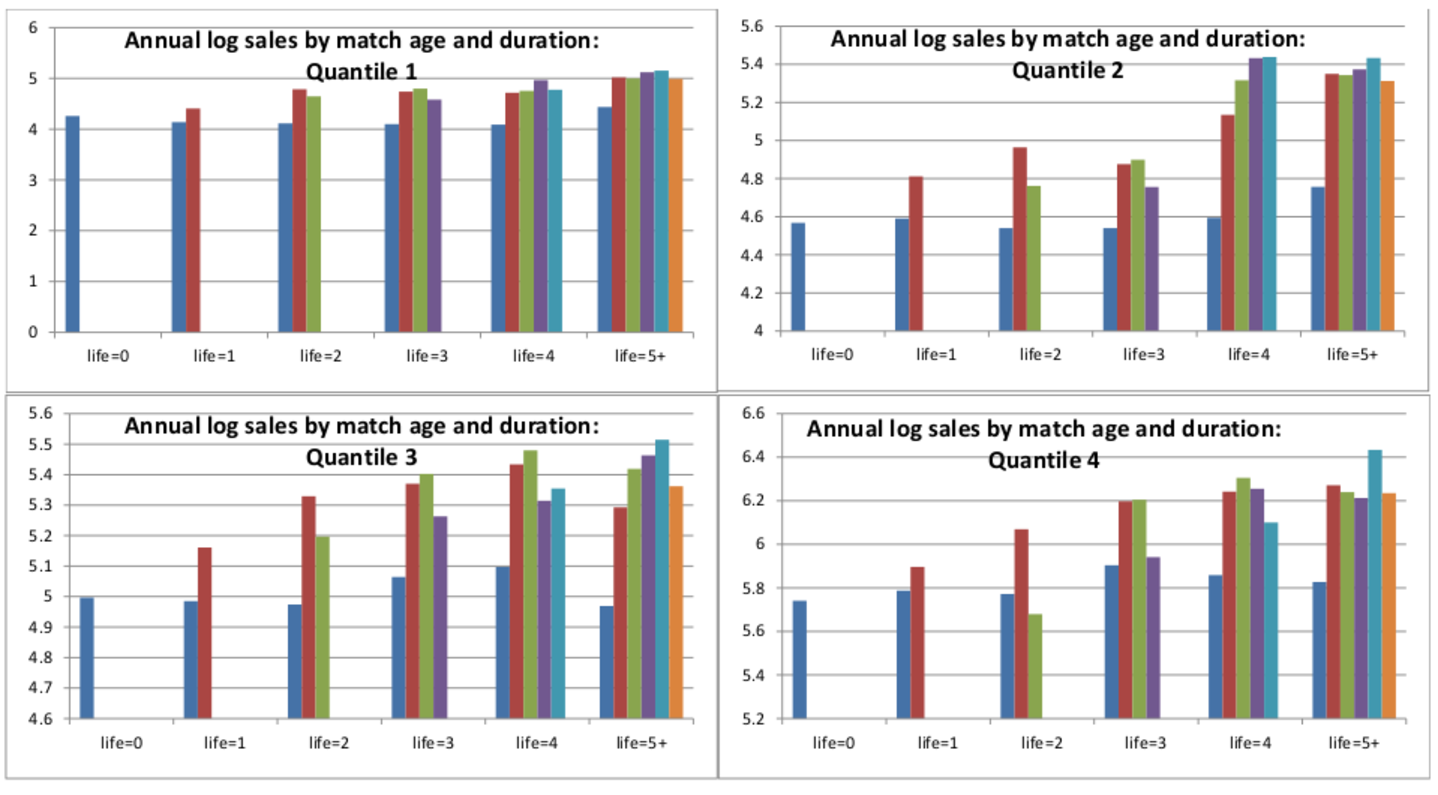
\includegraphics[width=\textwidth]{figures/figure1.pdf}
    \caption{\textbf{Average log annual sales per match, by initial size quartile}}
    \label{fig:match_maturation}
\end{figure}
\end{center}

The first message of these graphs is that initial sales are a good predictor
of sales in subsequent years, conditioning on survival. Those matches with
first-year sales in the smallest quartile systematically generated the
lowest annual sales in subsequent years, and more generally, first-year
sales are monotonically related to annual sales in subsequent years. Second,
sales tend to jump from the first to the second year, in large part simply
because observations on a match's first year correspond to less than a full
calendar year. (There is an analogous effect at work in the final year of a
match's life.) Looking at complete-year observations reveals a tendency for
annual sales to grow among matches that start small and survive, but no such
tendency among matches that start in the largest quartile. Finally, looking
across matches with different life spans, those that survive more years tend
to have higher sales in all (full) years than matches that fail relatively
quickly. This pattern is robust across matches in the different quartiles
for initial sales.

\subsubsection{Number of clients and sales per client}

Finally, firms that are successful at building a large client base also
manage to sell relatively large amounts to each client.\ To summarize this
relationship we fit the following regression:%
\begin{equation*}
\ln \overline{R}_{jt}=\phi _{0}^{r}+\phi _{1}^{r}\ln (n_{jt}^{c})+\phi
_{2}^{r}\ln (n_{jt}^{c})^{2}+\epsilon _{jt}^{r}
\end{equation*}%
Here $\overline{R}_{jt}$ is exporter $j^{\prime }$s average revenue per
client in year $t$, and $n_{jt}^{c}$ is the number of clients who received
shipments from $j$ during the same year. The regression implies $\overline{R}
$ is an increasing concave function of $n^{c}$: \ $\widehat{\phi }%
_{1}^{r}=2.67$; $\widehat{\phi }_{2}^{r}=-0.14.$

\section{A\ Model of Exporting at the Transactions Level}

We now develop a model of exporter behavior consistent with the patterns
reviewed above. Buyer-seller relationships form and disband at irregular
intervals. Similarly, export shipments are discrete events distributed
unevenly through time. To capture these features of the data, and to allow
agents to update their behavior each time their circumstances change, we
formulate our model in continuous time, treating all of the exogenous
processes in our model as Markov jump processes.

Explaining the evolution of a firm's exports and domestic sales requires
modeling both its sales to existing buyers and the evolution of its
portfolio of clients. We can treat these two components sequentially. We
first consider the relationship between a seller and an individual buyer.
Having characterized the seller's profits from a relationship with an
individual buyer, we then turn to her learning about the popularity of her
product, i.e., the chance that a potential buyers likes her product.
Finally, we characterize her search for buyers.





\subsection{A Seller-Buyer Relationship}

This section characterizes the profit streams that sellers generate from
successful business relationships. The expressions we develop here describe
relationships between domestic firms and foreign buyers, but with
appropriate relabelling of market-wide variables they apply equally to
relationships between domestic firms and domestic buyers.

\subsubsection{Profits from a single shipment}

Several features of our model are standard. First, at any time $t$ seller $j$
can hire workers at a wage $w_{t}$ in real local currency units, each of
whom can produce $\varphi _{j}$ $\in \{\varphi ^{_{1}},..,\varphi
^{_{N_{\varphi }}}\}$ units of output.\footnote{%
We treat $\varphi $ as time-invariant to facilitate model identification.
Other sources of idiosyncratic temporal variation in sales will be discussed
shortly.\medskip} \ Hence seller $j$'s unit cost in local currency is $%
w_{t}/\varphi _{j}.$ If she sells at price $p_{jt}$ in foreign currency her
unit profit in local currency is%
\begin{equation}
p_{jt}/e_{t}-w_{t}/\varphi _{j},  \label{unit profit}
\end{equation}%
where $e_{t}$ is the exchange rate. Second, goods markets are
monopolistically competitive and each producer supplies a unique
differentiated product.

Once buyer $i$ has agreed to form\ a business relationship with seller $j,$
he periodically places sales orders with $j$. For $j$, an order from $i$
that arrives at time $t$ generates revenue:%
\begin{equation}
X_{ijt}=\left( \frac{p_{jt}}{P_{t}}\right) ^{1-\eta }y_{ijt}\overline{X}_{t},
\label{demand}
\end{equation}%
where $\eta >1$ is buyers' elasticity of demand, $p_{jt}$ is the price of
seller $j$'s product, $\overline{X}_{t}$ is the average spending level among
all potential foreign buyers, $P_{t}$ is the relevant price index for all
competing products in the foreign market, and $y_{ijt}\in
\{y^{_{1}},..,y^{_{Ny}}\}$ is a time-varying demand shifter idiosyncratic to
the $ij$ relationship.\footnote{%
Not all buyers necessarily face the same range of goods and hence the same
aggregate price index $P$. We treat idiosyncratic components of the price
index as $P$ as reflected in $y_{ijt}.\medskip $}

For simplicity, and to keep the analysis as close as possible to other
heterogenous firm models, we assume that the seller posts a non-negotiable
price, charging the optimal markup over unit cost:\footnote{%
An alternative specification would introduce bilateral bargaining between
buyer and seller.\medskip}

\begin{equation}
p_{jt}=\frac{\eta }{\eta -1}\frac{e_{t}w_{t}}{\varphi _{j}}  \label{price}
\end{equation}%
By (\ref{unit profit}), (\ref{demand}), and (\ref{price}),\ an order from
buyer $i$ at time $t$ therefore generates the following profits for seller $%
j $:

\begin{equation*}
\pi _{ijt}=\frac{1}{\eta }\frac{\overline{X}_{t}}{e_{t}}\left( \frac{%
e_{t}w_{t}\eta /(\eta -1)}{\varphi _{j}P_{t}}\right) ^{1-\eta }y_{ijt}.
\end{equation*}

We can combine all the macroeconomic variables affecting the profit of any
seller from this source selling in this destination, along with constants,
as:%
\begin{equation*}
x_{t}=\frac{1}{\eta }\frac{\overline{X}_{t}}{e}\left( \frac{e_{t}w_{t}\eta
/(\eta -1)}{P_{t}}\right) ^{1-\eta },
\end{equation*}%
where $x\in \{x^{_{1}},..,x^{_{N_{x}}}\}$ is general to all potential buyers
in the foreign market. Suppressing subscripts on state variables, this
allows us to write the profits from a sale as:

\begin{equation}
\pi _{\varphi }(x,y)=x\varphi ^{\eta -1}y,  \label{profit2}
\end{equation}
\qquad \qquad

In what follows, (\ref{profit2}) is all we take from our specification of
preferences and pricing behavior into the dynamic analysis. Any set of
assumptions that deliver this simple multiplicative expression for a firm's
profit from a sale would serve us equally well.

\subsubsection{Relationship dynamics}

At any point in time, each seller maintains business relationships with an
endogenous number of buyers. These relationships form as a consequence of a
search process that will be characterized in the following section, and they
dissolve for several reasons. First, there is a constant exogenous hazard $%
\delta $ that any particular relationship will terminate, which could be due
to the demise of the buyer or the buyer no longer finding the seller's
product useful. Second, after each sale to a particular buyer, the seller
evaluates whether it is worth sustaining her relationship with him. Doing so
keeps the possibility of future sales to him alive, but it also means paying
the fixed costs $F$ of maintaining the account, providing technical support,
and maintaining client-specific product adjustments.\footnote{%
For instance, Colombian producers of construction materials interviewed for
a related project (Dom\'{\i}nguez et al, 2013) referred that it is frequent
for foreign buyers to request adjustments in the specifications of products
or packages. In turn, these require adjustments in the production process
that are costly to maintain.}

When deciding whether to maintain a particular business relationship, the
seller knows her own type, $\varphi $, the macro state, $x$ and profits from
the current sale, $\pi _{\varphi }(x,y)$ to the buyer in question. She can
therefore infer this buyer's current $y$ value and calculate the value of
her relationship with him to be:%
\begin{equation*}
\widetilde{\pi }_{\varphi }(x,y)=\pi _{\varphi }(x,y)+\max \left\{ \widehat{%
\pi }_{\varphi }(x,y)-F,0\right\} .
\end{equation*}%
Here $\widehat{\pi }_{\varphi }(x,y)$ is the expected value of continuing a
relationship that is currently in state $(x,y).$ Clearly the seller
terminates this relationship if $\widehat{\pi }_{\varphi }(x,y)$ $<F.$

If a seller pays $F$ to keep a relationship active, and if the relationship
does not end anyway for exogenous reasons, one of several events will next
affect it: with hazard $\lambda ^{b}$ the buyer will place another order,
with hazard $q_{xx^{\prime }}^{X}$ $x$ will jump to some new marketwide
state $x^{\prime }\neq x$, or with hazard $q_{yy^{\prime }}^{Y}$ $y$ will
jump to some new buyer-specific shock $y^{\prime }\neq y$.\footnote{ Since sales in the data are discrete events rather than flows, we model the
buyer's purchases accordingly. We think of the buyer not as making use of
the products continually but in discrete spurts. For example, the buyer
might be a producer of a product that it makes in batches. At the completion
of each batch it buys inputs for the next batch.\medskip} Let $\tau _{b}$ be
the random time that elapses until one of these events occurs. Given that $x$
and $y$ are Markov jump processes, $\tau _{b}$ is distributed exponentially
with parameter $\lambda ^{b}+\lambda _{x}^{X}+\lambda _{y}^{Y}, $ where%
\begin{equation}
\lambda _{x}^{X}=\sum_{x^{\prime }\neq x}q_{xx^{\prime }}^{X}  \label{q_K}
\end{equation}%
and%
\begin{equation}
\lambda _{y}^{Y}=\sum_{y^{\prime }\neq y}q_{yy^{\prime }}^{Y},  \label{q_Y}
\end{equation}%
are the hazards of transiting from $x$ to any $x^{\prime }\neq x,$ and from $%
y$ to any $y^{\prime }\neq y,$ respectively. Then assuming the seller has a
discount factor $\rho ,$ the continuation value $\widehat{\pi }_{\varphi
}(x,y)$ solves the Bellman equation:%
\begin{eqnarray*}
\widehat{\pi }_{\varphi }(x,y) &=&\mathbf{E}_{\tau _{b}}\left[ e^{-(\rho
+\delta )\tau _{b}}\frac{1}{\lambda ^{b}+\lambda _{x}^{X}+\lambda _{y}^{Y}}%
\left( \sum_{x^{\prime }\neq x}q_{xx^{\prime }}^{X}\widehat{\pi }_{\varphi
}(x^{\prime },y)+\sum_{y^{\prime }\neq y}q_{yy^{\prime }}^{Y}\widehat{\pi }%
_{\varphi }(x,y^{\prime })+\lambda ^{b}\widetilde{\pi }_{\varphi
}(x,y)\right) \right] \\
&=&\frac{1}{\rho +\delta +\lambda ^{b}+\lambda _{x}^{X}+\lambda _{y}^{Y}}%
\left( \sum_{x^{\prime }\neq x}q_{xx^{\prime }}^{X}\widehat{\pi }_{\varphi
}(x^{\prime },y)+\sum_{y^{\prime }\neq y}q_{yy^{\prime }}^{Y}\widehat{\pi }%
_{\varphi }(x,y^{\prime })+\lambda ^{b}\widetilde{\pi }_{\varphi
}(x,y)\right)
\end{eqnarray*}

Before a seller has met her next buyer, she does not know what state $y$
this buyer will happen to be in. So when choosing her search intensity for
new business relationships, she must base her decisions on the ex ante
expected pay-off to forming a new business relationship. Given the market
state $x$, a type-$\varphi $ seller calculates this expected value as:%
\begin{equation*}
\widetilde{\pi }_{\varphi }(x)=\sum_{s}\Pr (y^{s})\widetilde{\pi }_{\varphi
}(x,y).
\end{equation*}%
where $\Pr (y^{s})$ is the probability that a randomly selected buyer is
currently in state $y^{s}\in \{y^{_{1}},..,y^{_{Ny}}\}$.\footnote{%
Here we take the probabilities $\Pr (y^{m})$ to be the ergodic distribution
of $y$ implied by the transition hazards $q_{yy^{\prime }}^{Y}.$ We could
assume that the distribution at the time of the first purchase is different
from the ergodic one.\medskip}

For the purposes of the search model that follows, all that matters about an
individual relationship is $\widetilde{\pi }_{\varphi }(x),$ and this object
can be estimated directly from data on the revenue streams generated by
matches. Nonetheless, the history of a seller's interactions with a given
buyer affects its overall sales trajectory and hence matters for our
characterization of aggregate export dynamics.

Hereafter, we will denote the expected value of a relationship with a
foreign buyer by $\widetilde{\pi }_{\varphi }^{f}(x)$ and the expected value
of a relationship with a home market buyer by $\widetilde{\pi }_{\varphi
}^{h}(x).$ These two objects are calculated in the same way, but since
expenditure levels ($\overline{X}_{t}$) and price indices ($P_{t}$) differ
across markets, and no exchange rate factor $e$ is necessary for domestic
profit calculations, each has its own process for the market-wide state
variable, $x.$ These market-wide demand shifters are denoted $x^{f}$ and $%
x^{h}$ below$.$

\subsection{Learning about Product Appeal}

Sellers conduct market-specific searches for buyers. When searching in
market $m\in \{h,f\}$, each recognizes that some fraction $\theta ^{m}$ $\in
\lbrack 0,1]$ of the potential buyers she meets there will be willing to do
business with her. An encounter with one of these willing buyers generates
an expected profit stream worth $\widetilde{\pi }_{\varphi ,x}^{m}$, while
an encounter with any of the remaining potential buyers does not generate a
sale then or subsequently.

Each seller's $\theta ^{h}$ and $\theta ^{f}$ values are drawn before she
has met any clients. These draws remain fixed through time, inducing
permanent cross-market differences in her product's popularity. All $\theta
^{m}$ draws are independently beta-distributed across sellers and markets:%
\begin{equation*}
b(\theta ^{m}|\alpha ,\beta )=\frac{\Gamma (\alpha +\beta )}{\Gamma (\alpha
)\Gamma (\beta )}\left( \theta ^{m}\right) ^{\alpha -1}(1-\theta
^{m})^{\beta -1},\;m\in \{h,f\},
\end{equation*}%
where $\Gamma (\phi )=\int_{0}^{\infty }z^{\phi -1}e^{-z}dz$ is the gamma
function (needed to ensure that the distribution has the proper limits).
However, the independence of $\theta ^{h}$ and $\theta ^{f}$ does not mean
sellers' domestic and foreign sales are likewise independent. Rather,
cross-market correlation in sales will be induced by\ the firm type $\varphi
,$ which can be viewed as capturing aspects of product appeal that are
common to both markets$.$\footnote{%
The firm effect is similarly interpreted to reflect both productive
efficiency and product appeal in Melitz (2003) and many other papers based \
on CES demand systems. However in the present context, the global aspects of
product appeal captured by $\varphi $ are qualitatively distinct from the
market-specific product appeal effects captured by $\theta $. The former
determines the amount of a product each buyer purchases, given that he is
interested, while the latter determines what fraction of potential buyers
are willing to place orders with the seller, should they happen to meet
her.\medskip}

Sellers are presumed to have already met many potential customers in the
domestic market, and thus to have learned their $\theta ^{h}$ draws. But
sellers typically have far less experience abroad, so we allow them to still
be learning about their $\theta ^{f}$ draws. Specifically, each seller
recognizes that for any given $\theta ^{f},$ the probability a random sample
of $n$ potential foreign buyers will yield $a$ customers is binomially
distributed: 
\begin{equation*}
q\left[ a|n,\theta ^{f}\right] =\binom{n}{a}\left[ \theta ^{f}\right] ^{a}%
\left[ 1-\theta ^{f}\right] ^{n-a}.
\end{equation*}%
So after she has met $n$ potential buyers abroad, $a$ of whom were willing
to buy her product, a seller's posterior beliefs about her $\theta ^{f}$
draw are distributed:%
\begin{equation*}
p(\theta ^{f}|a,n)\propto q\left[ a|n,\theta ^{f}\right] \cdot b(\theta
^{f}|\alpha ,\beta )
\end{equation*}%
where the factor of proportionality is the inverse of the integral of the
right-hand side over the support of $\theta^{f}$. Since the beta distribution
is the conjugate prior for the binomial, a firm's expected success rate
after $a$ successes in $n$ trials has a convenient closed-form
representation: 
\begin{equation}
\overline{\theta }_{a,n}^{f}=E\left[ \theta ^{f}|a,n\right]
=\int_{0}^{1}\theta p(\theta |a,n)d\theta =\frac{a+\alpha }{n+\alpha +\beta }%
.  \label{success_probability}
\end{equation}%
This posterior mean converges to $p\lim \left( \frac{a}{n}\right) =\theta
^{f}$ as $n$ gets large.

\subsection{Searching for Buyers}

To complete our model we now consider sellers' search intensities in each
market. Each seller continuously chooses the market-specific hazard $s^{m},$ 
$m\in \{h,f\},$ with which she encounters a potential buyer, recognizing
that this involves the instantaneous flow cost $c(s^{m},a),$ where $%
c(s^{m},a)$ is increasing and convex in $s^{m}.$\footnote{%
Interviews conducted with Colombian exporters revealed a variety of
activities firms pursue to meet potential buyers abroad (Dom\'{\i}nguez, et
al, 2013). Ranked roughly in terms of decreasing cost, these included
maintaining a foreign sales office; paying the exports promotion office to
organize visits with prospective clients abroad, and sending their sales
representatives to those visits; sending sales representatives abroad to
visit potential clients on their own; attending trade fairs; paying a
researcher to search the web for foreign firms that purchase products
similar to their own; paying browsers to ensure that their site appear near
the top of a search for their product type; maintaining a web site in
English.\medskip\ Interviewees also reported that relatively low-cost
activities, such as traveling to trade fairs, or translating their websites
to English, led to relationships with one or two clients every few years.
Establishing a larger network of clients required much more costly
activities.} Whether $c(s^{m},a)$ increases or decreases in the number of
successful matches, $a,$ depends upon the relative strength of several
forces and will be left for the data to determine. Costs might fall with $a$
because encounters with interested buyers increase the seller's visibility
and enhance her opportunities to meet additional potential buyers.
Alternatively, costs might rise if the pool of easy-to-reach buyers becomes
"fished out," as in Arkolakis\ (2007).

We can now describe optimal search behavior, beginning with the foreign
market. Recall that when the foreign market state is $x^{f}$, a type-$%
\varphi $ seller expects the value of a new business relationship will be $%
\widetilde{\pi }_{\varphi }^{f}(x^{f}).$ Further, she believes the next
match will yield such a relationship with probability $\overline{\theta }%
_{a,n}^{f}$. Combined with search cost function $c(s^{f},a)$ and the jump
process for $x^{f}$, these objects imply sellers' optimal search policy
abroad.

To characterize this policy, let $\tau _{s}^{f}$ be the random time until
the next foreign search event, which could be either a change in the
marketwide state $x^{f}$ or an encounter with a potential buyer. Then,
suppressing market superscripts, the optimal search intensity $s$\ for a
type-$\varphi $ firm with foreign market search history $(a,n)$ solves the
following the Bellman equation:%
\begin{eqnarray*}
&&V_{\varphi }(a,n,x)=\max_{s}\mathbf{E}_{\tau _{s}}\left[
-c(s,a)\int_{0}^{\tau _{s}}e^{-\rho t}dt+\frac{e^{-\rho \tau _{s}}}{%
s+\lambda _{x}^{X}}\cdot \left( \sum_{x^{\prime }\neq x}q_{xx^{\prime
}}^{X}V_{\varphi ,}(a,n,x^{\prime })\right. \right. \\
\; &&\left. \left. 
\begin{array}{c}
\; \\ 
\;%
\end{array}%
+s\left[ \overline{\theta }_{a,n}(\widetilde{\pi }_{\varphi }(x)+V_{\varphi
}(a+1,n+1,x)+(1-\overline{\theta }_{a,n})V_{\varphi }(a,n+1,x)\right]
\right) \right]
\end{eqnarray*}%
(Recall that $\lambda _{x}^{X}$ is given by (\ref{q_K}).) Taking
expectations over $\tau _{s}$ yields:%
\begin{eqnarray}
V_{\varphi }(a,n,x) &=&\max_{s}\frac{1}{\rho +s+\lambda _{x}^{X}}\left[
-c(s,a)+\sum_{x^{\prime }\neq x}q_{xx^{\prime }}^{X}V_{\varphi
,}(a,n,x^{\prime })\right.  \label{V_search2} \\
&&\left. 
\begin{array}{c}
\; \\ 
\;%
\end{array}%
+s\left\{ \overline{\theta }_{a,n}\left[ \widetilde{\pi }_{\varphi
}(x)+V_{\varphi }(a+1,n+1,x)\right] +(1-\overline{\theta }_{a,n})V_{\varphi
}(a,n+1,x)\right\} \right]  \notag
\end{eqnarray}%
Applying the multiplication rule for differentiation and using expression (%
\ref{V_search2}) for $V_{\varphi }(a,n,x)$, the optimal search intensity $%
s^{\ast }$ satisfies:%
\begin{equation}
\frac{\partial c(s^{\ast },a)}{\partial s}=\overline{\theta }_{a,n}\left[ 
\widetilde{\pi }_{\varphi }(x)+V_{\varphi }(a+1,n+1,x)\right] +(1-\overline{%
\theta }_{a,n})V_{\varphi }(a,n+1,x)-V_{\varphi }(a,n,x)
\label{FOC_MS_learning}
\end{equation}%
That is, the marginal cost of search must equal the expected marginal
benefit of a match, which includes the expected value of the associated
profit stream, $\overline{\theta }_{a,n}\widetilde{\pi }_{\varphi }(x)$, and
the expected value of the information generated.

Now consider the home market. Since we assume sellers have already learned
their true success rates at home, $\theta ^{h},$ new encounters do not
influence expectations, and we need not condition the value function or the
expected success rate on search histories$.$ Again suppressing market
superscripts, the Bellman equation collapses to:%
\begin{equation}
V_{\varphi }(x)=\max_{s}\frac{1}{\rho +\lambda _{x}^{X}}\left[
-c(s,a)+\sum_{x^{\prime }\neq x}q_{xx^{\prime }}^{X}V_{\varphi }(x^{\prime
})+s\theta _{j}\widetilde{\pi }_{\varphi }(x)\right]  \notag
\end{equation}%
and the first-order condition is simply:%
\begin{equation*}
\frac{\partial c(s^{\ast },a)}{\partial s}=\theta _{j}\widetilde{\pi }%
_{\varphi }(x).
\end{equation*}%
The marginal cost of search equals the expected profit from a successful
relationship times the probability of success.

\section{An empirical version of the model}

\subsection{The search cost function}

To implement our model empirically, we impose additional structure in
several respects. First, we specify a functional form for our search cost
function. Generalizing Arkolakis\ (2007) to allow for network effects, we write these costs as:%
\begin{equation}
c(s,a)=\kappa _{0}\frac{\left[ (1+s)\right] ^{(1+1/\kappa _{1})}-1}{%
(1+a)^{\gamma (1+1/\kappa _{1})}(1+1/\kappa _{1})}.  \label{cost of effort}
\end{equation}%
Several properties of this function merit note. First, marginal costs fall
at a rate determined by $\gamma $ with the number of successful matches a
seller has already\ made, so $\gamma >0$ implies \textquotedblleft
network\textquotedblright\ effects and $\gamma <0$ implies "congestion"
effects.\footnote{%
To contain the dimensionality of the computational problem we solve, we
assume that firms with more than $a^{\ast }$ buyers have (i) exhausted their
learning effects, and (ii) reap no additional network effects at the margin
from further matches. We choose $a^{\ast }$ to exeed the observed maximum $a$
for 99 percent of sellers in the foreign (United States) market. Also, we
set $a=a^{\ast }$ for all sellers in their home (Colombian) market.\medskip}
Second, a seller who is not searching in a particular market incurs no
search cost: $c(0,a)=0.$ Third, given the cumulative number of successful
matches, $a,$ the marginal cost of search increases with $\lambda ^{s}$ at a
rate inversely related to $\kappa _{1}:$ $c_{s}(s,a)$ $=$ $\kappa _{0}\left[
(1+s)/(1+a)^{\gamma }\right] ^{1/\kappa _{1}}.$ Finally, network effects
endure, even if a firm is not actively searching.

\subsection{Processes for exogenous state variables}

Next we impose more structure on the exogenous state variables, $\varphi ,$ $%
x^{h},$ $x^{f},$ $y^{h}$ and $y^{f}.$ All are assumed to have zero means in
logs, and the net effect of these normalizations is undone by introducing
scalars $\Pi ^{h}$ and $\Pi ^{f}$ into the home and foreign profit
functions, respectively:%
\begin{eqnarray*}
\pi _{\varphi }^{f}(x^{f},y^{f}) &=&\Pi ^{f}x^{f}\varphi ^{\eta -1}y^{f}, \\
\pi _{\varphi }^{h}(x^{h},y^{h}) &=&\Pi ^{h}x^{f}\varphi ^{\eta -1}y^{f}
\end{eqnarray*}

More substantively, we impose that the cross-firm distribution of $\varphi $
is log normal with standard deviation $\sigma _{\varphi },$ and we treat all
of the Markov jump processes $(x^{h},y^{h},x^{f},y^{f})$ as independent
Ehrenfest diffusion processes. The idiosyncratic match shocks, $y^{f}$ and $%
y^{h},$ are assumed to share the same distribution, but we allow the $x^{f}$
and $x^{h}$ processes to differ. Among other things, the latter accommodates
the fact that the exchange rate affects aggregate demand and price indices
in the two markets differently.

Any variable $z$ generated by an Ehrenfest process can be discretized into $%
2g+1$ possible values, $g\in I^{+}:$ $z\in \{-g\Delta ,$ $-(g-1)\Delta ,$ $%
..,$ $0,..,$ $(g-1)\Delta ,$ $g\Delta \}.$ Further, it jumps to a new value
with hazard $\lambda _{z},$ and given that a jump occurs, it goes to $%
z^{\prime }$ according to:

\begin{equation*}
z^{\prime }=\left\{ 
\begin{array}{c}
z+\Delta \\ 
z-\Delta \\ 
\text{other}%
\end{array}%
\right. \text{with probability }\left\{ 
\begin{array}{c}
\frac{1}{2}\left( 1-\frac{z}{g\bigtriangleup }\right) \\ 
\frac{1}{2}\left( 1+\frac{z}{g\bigtriangleup }\right) \\ 
0%
\end{array}%
\right. .
\end{equation*}%
Thus, given a grid size $g$, the intensity matrices $Q^{X}=\left\{
q_{ij}^{X}\right\} _{i,j=1,N^{X}}$ and $Q^{Y}=\left\{ q_{ij}^{Y}\right\}
_{i,j=1,N^{Y}}$ that were introduced in section 3.1 are each block-diagonal
and characterized by a single parameter, $\Delta $.

\section{Estimation}

\subsection{Stage 1: estimating observable jump processes}

Shimer (2005) shows that if $z$ follows a continuous time Ehrenfest
diffusion process, it asymptotes to an Ornstein-Uhlenbeck process with mean
zero as the fineness of the grid increases:\footnote{%
Specifically, replacing the parameter vector $(\lambda ,g,\Delta )$ with $%
(\lambda /\epsilon ,g/\epsilon ,\Delta \sqrt{\epsilon }),$ $\epsilon >0,$
leaves the autocorrelation parameter $\mu $ and the instantaneous variance
parameter $\sigma $ unchanged. But as $\epsilon \rightarrow 0,$ the
innovation $dW$ $\ $approaches normal.\medskip} 
\begin{equation*}
dz=-\mu zdt+\sigma dW.
\end{equation*}%
Here $\mu =\lambda _{z}/g$, $\sigma =\sqrt{\lambda _{z}}\Delta $, and $W$
follows a Weiner process. Accordingly, since it is possible to observe
proxies for $x^{f}$ and $x^{h}$, these can be viewed as discrete time
observations on underlying Ornstein-Uhlenbeck processes, and the parameters
of these processes can be econometrically estimated. Then, given $\mu $ and $%
\sigma ,$ estimates of $\Delta $ and $\lambda $ for these processes can be
inferred.

\begin{table}
    \centering
    \begin{tabular}{lll}
        \multicolumn{3}{c}{\textbf{}} \\ 
        \hline\hline
        & \textit{Parameter} & \textit{value} \\ \hline
        home macro state jump hazard    & $\lambda ^{x_{h}}$ & \multicolumn{1}{c}{1.200}  \\
        foreign macro state jump hazard & $\lambda ^{x_{f}}$ & \multicolumn{1}{c}{ 1.215} \\
        home macro state jump size      & $\Delta ^{x_{h}}$  & \multicolumn{1}{c}{0.003}  \\
        foreign macro state jump size   & $\Delta ^{x_{f}}$  & \multicolumn{1}{c}{0.053}  \\ \hline
    \end{tabular}%
    \caption{\textbf{Market-wide Demand Shifters}}
    \label{tab:dem_shift}
\end{table}


Measuring $x^{f}$ as real expenditures on manufacturing goods in the U.S.,
and measuring $x^{h}$ as real expenditures on manufacturing goods in
Colombia, we obtain the results reported in Table \ref{tab:dem_shift}.%
\footnote{%
Our foreign market size mesaure is the OECD time series on American GDP in 'Industry, including
energy' adding imports and subtracting net exports of manufactures. Our home market size measure
is real Colombian expenditures on manufacturing goods, taken from DANE. 
We converted all of the data used for the estimation into real 1992 US
dollars, deflating nominal US dollars with the consumer price index available on
 the US Bureau of Labor Statistic website. We used an
official Colombian Peso - US Dollar exchange rate time series downloaded
from the Central Bank of Colombia to convert Pesos to nominal US Dollars} They imply that $x^{f}$ and $x^{h}$ both jump 1.2 times per year, on
average. However, jumps in the U.S. market tend to be much larger,
essentially because they reflect movements in the real exchange rate as well
as movement in dollar-denominated expenditures.

\subsection{Stage 2: Indirect inference}

Our data are relatively uninformative about the rate of time discount $\rho $
and the demand elasticity $\eta $, so we do not attempt to estimate either
one$.$ For the former we follow convention and assume $\rho =0.05$. For the
latter, following many previous trade papers, we fix the demand elasticity
at $\eta =5.$ All of the remaining parameters we estimate using the method
of indirect inference (Gouri\'{e}roux and Monfort, 1996). These parameters
include the exogenous match separation hazard (${\small \delta }$), the
market size scalars (${\small \Pi }^{h},{\small \Pi }^{f.}$), the fixed
costs of maintaining a match ($F$), the parameters of the product appeal
distributions (${\small \alpha }{\small ,}{\small \beta }$), the dispersion
of the productivity distribution ($\sigma _{\varphi }$), the jump hazards
for the idiosyncratic buyer shocks ($\lambda _{y}$), the hazard rate for
shipments (${\small \lambda }_{b}$), the network/congestion parameter ($%
\gamma $), the cost function convexity parameter (${\small \kappa _{1}}$),
and the cost function scaling parameter (${\small \kappa _{0}}$). \textbf{\ }%
For notational convenience we hereafter collect these parameters in the
vector $\Lambda :$%
\begin{equation*}
\Lambda =\left( {\small \Pi }^{h},{\small \Pi }^{f.},{\small \delta ,}F,%
{\small \alpha },{\small \beta },\sigma _{\varphi },\lambda _{y},{\small %
\lambda }_{b},{\small \gamma ,\kappa _{0},\kappa _{1}}\right)
\end{equation*}

We seek the value of $\Lambda $ that allows our model to replicate the
features of the transactions-level data summarized in Section \ref{sec:data} above. In
addition to the joint distribution of home and foreign sales across firms,
these include the distribution of clients across exporters, the
probabilities than a particular exporter will move up or down in this
distribution, given its current position, the hazard that a given match will
end, given its current age and size, the survival rates of exporting cohorts
as they mature, and the distribution of shipment frequencies across matches.

% \renewcommand{\familydefault}{\sfdefault}
\begin{table}[tbp] 
\renewcommand{\arraystretch}{1.2}
%\begin{tabular}{lll}
    \begin{tabular}{lrrr} \hline \hline 
\textbf{Data feature} & \textbf{Summary method } & \textbf{Statistics (}$\widehat{M}$\textbf{)} \\ \noalign{\smallskip} \hline \noalign{\smallskip}
Distribution of home & OLS cross-plant regression: &  \\
and foreign sales & $\ln X_{jt}^{f}$ = $\phi _{0}^{hf}+\phi _{1}^{hf}\ln
X_{jt}^{h}+\epsilon _{jt}^{hf}$ & $\widehat{\phi }_{0}^{hf}$, $\widehat{\phi 
}_{1}^{hf}$, $s\widehat{e}(\epsilon ^{hf})$ \\ 
& Cross-plant moments & $\widehat{E}(1_{X_{jt}^{f}>0}),\widehat{E}(\ln
X_{jt}^{f}|X_{jt}^{f}>0),$ \\ 
& Standard deviation of foreign sales & $se(\ln X_{jt}^{f})$ \\ \noalign{\smallskip} \hline \noalign{\smallskip} 
Distribution of clients & OLS regression for $n^{c}\in I^{+}$ : &  \\ 
across exporters, $\Phi (n^{c})$ & $\ln \left[ 1-\Phi (n^{c})\right] =\phi
^{c}\ln (n^{c})+\epsilon ^{n}$ & $\widehat{\phi }^{c},$ $s\widehat{e}%
(\epsilon ^{n^{c}})$ \\ \noalign{\smallskip} \hline \noalign{\smallskip}
Sales per client given & OLS cross-match regression: $\ln X_{ijt}^{f}=$ & 
\\
number of clients & $\phi _{0}^{r}+\phi _{1}^{r}\ln (n_{jt}^{c})+\phi
_{2}^{r}\ln (n_{jt}^{c})^{2}+\epsilon ^{m}$ & $\widehat{\phi }_{0}^{r}$, $%
\widehat{\phi }_{1}^{r}$, $\widehat{\phi }_{2}^{r},$ $s\widehat{e}(\epsilon
^{r})$ \\ \noalign{\smallskip} \hline \noalign{\smallskip}
Autoregression, & &  \\ 
log domestic sales & $\phi _{0}^{h}+\phi _{1}^{h}\ln X_{jt-1}^{h}+\epsilon ^{h}$
 & $\widehat{\phi }_{1}^{h},$ $s\widehat{e}(\epsilon ^{h})$ \\ \noalign{\smallskip} \hline \noalign{\smallskip}
Transition probabilities, & Cross-plant year-to-year & $\widehat{P}%
[n_{jt+1}^{c}=m|n_{jt}^{c}=k],$ \\ 
number of clients $(n_{jt}^{c})$ & average transition rates & $m,k=0,1,2,3+$
\\ \noalign{\smallskip} \hline \noalign{\smallskip}
Match death hazards, & Cross-match average & $\widehat{E}%
[1_{X_{ijt}^{f}=0}|X_{ijt-1}^{f}>0,A_{ijt-1}^{m}],$ \\ 
given match age $(A^{m})$ & year-to-year death rates, given age & $%
A_{ijt-1}^{m}=0,1,2,3,4+$ \\ \noalign{\smallskip} \hline \noalign{\smallskip}
Exporter exit hazard & Cross exporter average exit rate, & $\widehat{E}%
[1_{X_{jt}^{f}=0}|A_{jt}^{c}],$ \\ 
by cohort age $(A^{c})$ & given years exporting & $A_{jt}^{c}=0,1,2,3,4+$ \\ \noalign{\smallskip} \hline \noalign{\smallskip}
Cohort-specific & Cross-exporter mean log exports & $\widehat{E}(\ln
X_{jt}^{f}|A_{jt}^{c}),$ \\ 
exports per plant &  & $A_{jt}^{c}=1,2,3,4+$ \\ \noalign{\smallskip} \hline \noalign{\smallskip}
Match-specific shipments & Cross-match mean &  \\ 
per year $(n_{ijt}^{s})$ & shipments per year & $\widehat{E}\left(n^{s}\right) $ (trimmed) \\ \noalign{\smallskip} \hline \noalign{\smallskip}
Autoregression, match- &  & \\
specific sales ($X_{ijt}^{f}$) & $\ln X_{ijt}^{f}=\widehat{\beta }_{0}^{f}+\widehat{%
\beta }_{1}^{f}\ln X_{ijt-1}^{f}+\epsilon _{ijt}^{f}$ & $\widehat{\beta }_{1}^{f},$ $s\widehat{e}(\epsilon ^{f})$ \\ \noalign{\smallskip} \hline \noalign{\smallskip}
Match death prob. & $1_{X_{ijt}^{f}=0}=\widehat{\beta }_{0}^{d}+\widehat{%
\beta }_{\mbox{1st year}}^{d}1_{A_{ijt-1}^{m}=0}$ &  \\ \noalign{\smallskip}
and match sales & $+\widehat{\beta }_{\mbox{lsales}}^{d}\ln
X_{ijt-1}^{f}+\epsilon _{ijt}^{d}$ & $\widehat{\beta }_{0}^{d},\widehat{\beta }_{\mbox{1st year}}^{d},\widehat{\beta }_{%
\mbox{lsales}}^{d},s\widehat{e}(\epsilon ^{d})$ \\ \noalign{\smallskip} \hline \noalign{\smallskip}
\end{tabular}%
\newline\flushleft\small{\small Variable definitions: }

$n_{jt}^{c}${\small : number of foreign clients served by firm }$j${\small \ in year }${\small t}${\small \ }

${\small \Phi }{\small (n^{c})}:${\small \ cumulative frequency distribution of number of foreign clients in population of exporters }

$A_{ijt}^{m}:${\small \ age of match (in years) between seller }${\small j}${\small \ and foreign buyer }${\small i}${\small \ in year }${\small t} ${\small \ }

$A_{jt}^{c}${\small : number of consecutive years exporter }$j${\small \ has
made at least one shipment abroad.}
\caption{\textbf{Statistics used for Indirect Inference}}
\label{tab:ind_inf_stats}
\end{table}%
% $^{\dag}$} \\ \noalign{\smallskip} \hline \noalign{\smallskip} \noalign{\smallskip} \hline
%EndExpansion
%EndExpansion
\renewcommand{\arraystretch}{1}

The sample statistics that we use as a basis for inference are listed in
Table \ref{tab:ind_inf_stats}. These same statistics are also repeatedly constructed using data
simulated with the model at alternative candidate values for $\Lambda $. The
method of indirect inference amounts to choosing the $\Lambda $ value that
minimizes a metric of the distance between sample and simulated 
statistics.\footnote{More precisely, our estimator for $\Lambda $ is: 
\begin{equation*}
\widehat{\Lambda }=\arg \min \left[ \widehat{M}-M_{S}(\Lambda )\right]
^{\prime }\widehat{W}^{-1}\left[ \widehat{M}-M_{S}(\Lambda )\right]
\end{equation*}%
where $\widehat{M}$ is the vector of data-based statistics listed in the
right-most column of Table \ref{tab:ind_inf_stats}, $M_{S}(\Lambda )$ is their counterpart based
on $S$ simulations of our model at candidate vector $\Lambda ,$ and $%
\widehat{W}$ is a compatible matrix with $\widehat{se}(\widehat{M})$ on its
diagonal and zeros elsewhere. These standard errors are constructed using
the sample data. In addition to giving the greatest weight to those
statistics that are most precisely estimated, $W^{-1}$ serves to eliminate
units of measurement as a factor in determining the fit.
The efficient GMM estimator of $\phi $ would use $E\left[ \widehat{M}-E(%
\widehat{M})\right] \left[ \widehat{M}-E(\widehat{M})\right] ^{\prime }$
(adjusted for simulation error in $M(\Lambda )$) as its weighting matrix.
But since our data on establishments and matches come from several sources,
it computationally infeasible for us to construct this set of weights. Our
weighting matrix yields a consistent estimator, provided that our model is
properly specified.}


While there is no exact mapping between the statistics in the last column of
Table \ref{tab:ind_inf_stats} and the parameters we wish to estimate, it is possible to comment in
general terms on sources of identification. First, several parameters are
closely associated with sample means. Specifically, the profit function
scaling parameters $\Pi ^{h}$ and $\Pi ^{f}$ are identified by average
levels of sales in each market, $E(\ln X_{jt}^{h})$ and $E(\ln X_{jt}^{f}),$
given market participation, as well as the fraction of firms that export, $%
E(1_{X_{jt}^{f}>0})$. And the shipment hazard $\lambda _{b}$ is closely
related to the average number of shipments per year, $\widehat{E}\left(
n^{s}\right) .$

Second, the match-specific shock hazard, ${\small \lambda }^{y},$ the
exogenous match separation hazard, $\delta ,$ and the fixed costs of
maintaining a match, $F,$ are key determinants of the persistence and
dispersion in client-specific sales trajectories. Accordingly, key
statistics that help to identify these parameters include estimates of
autoregressions for match-specific sales $\widehat{\beta }_{1}^{f},$ $s%
\widehat{e}(\epsilon ^{f})$, match death hazards by age of match, $\widehat{E%
}[1_{X_{ijt}^{f}=0}|X_{ijt-1}^{f}>0,A_{ijt-1}^{m}],$ and parameters of the
regression relating match death hazards to match size: $\widehat{\beta }%
_{0}^{d},\widehat{\beta }_{\mbox{1st year}}^{d},\widehat{\beta }_{%
\mbox{lsales}}^{d},s\widehat{e}(\epsilon ^{d}).$ Since the fixed costs of
sustaining a match are incurred after each shipment, the difference in
separation hazards between the first and all subsequent years helps to
distinguish $F$ from $\delta .$ Also, in the absence of shocks to
market-wide conditions ($x$) or idiosyncratic buyer demands ($y$), all
matches would survive $A$ periods with probably $(1-\delta )^{A}.$
Accordingly, the rate at which hazard rates decline with match age is
informative about $\delta .$ Further identification comes from the fact that 
$\delta $ affects all firms equally, while the effect of $F$ declines as $%
\widehat{\pi }_{\varphi ,x}$ increases. This makes the association between
shipment size and match longevity informative regarding the importance of $%
F. $

Third, the $\theta $ distribution parameters, $\alpha $ and $\beta $,
determine the cross-firm joint distribution of success rates in home and
foreign markets and, similarly, the dispersion in firm types $\sigma
_{\varphi }$ helps determine the cross-distribution of domestic and foreign
sales.\ The combined effects of these parameters is reflected in the means,
variances, and covariances of foreign and domestic sales, which are implied
in turn by $\widehat{\phi }_{1}^{hf}$, $s\widehat{e}(\epsilon ^{hf}),$ and $%
se(\ln X_{jt}^{f}).$ Similarly, the cross-firm distribution of numbers of
foreign clients, summarized by $\widehat{\phi }^{c}$ and $s\widehat{e}%
(\epsilon ^{n^{c}}),$ responds to ($\alpha $,$\beta )$. This distribution
also responds to $\sigma _{\varphi },$ since the firm effects $\varphi $
strongly influence search intensities. But the role of the firm effects $%
\varphi $ is distinct from that of the popularity indices $\theta ^{f}$ and $%
\theta ^{h}$\ because $\varphi $ induces correlation in sales across
markets. This correlation, which is implied by $\widehat{E}(\ln
X_{jt}^{f}|A_{jt}^{c})$, $\widehat{\phi }_{1}^{hf}$, $s\widehat{e}(\epsilon
^{hf}),$ and $se(\ln X_{jt}^{f})$, helps to isolate the variance in firm
effects, $\sigma _{\varphi }.$

Finally, the marginal cost of search and its sensitivity to previous matches
are determined by ${\normalsize \gamma ,\kappa }_{0}{\normalsize ,}$ and $%
{\normalsize \kappa }_{1}$. Match rates, transition probabilities for
numbers of clients, $\widehat{P}[n_{jt+1}=m|n_{jt}=k],$ and the client
distribution are informative about the convexity of the matching cost
function. Accordingly, $\widehat{\beta }^{c}$ and $s\widehat{e}(\epsilon
^{n})$ are useful in their identification. Differences in match arrival
rates among firms that have made many versus few matches help to distinguish
the convexity parameter $\beta $ from the network effect parameter, $\gamma
. $ And importantly, the shape of the client-per-seller distribution is
informative about network effects, since these effects critically impact the
ability of firms to sustain large client bases, and thus affect the
"fatness" of the right-hand tail.

\subsection{Parameter estimates}

Table \ref{tab:est_results} reports estimates based on the data moments described in the
previous subsection. Data-based estimates of these moments, $\widehat{M},$
are reported and juxtaposed with their simulated counterparts, $%
M_{S}(\Lambda )$, in Table \ref{tab:est_results}.\footnote{%
The share exporters, the coefficient of log foreign sales on log domestic
sales, and the AR1 coefficient for log domestic sales in Table \ref{tab:est_results} are
obtained from a combination of the Colombian Annual Manufacturing Survey
(AMS) and the administrative records of exports transactions. The data used
cover 1993-2007. Exports from administrative records are merged into the AMS
using firm identifiers. This is done because the AMS has no export
information for 1993-1999, and because the dynamics of aggregate exports
reported in the EAM starting in 2004 differ substantially from aggregate
reports from other sources.} The Euclidean distance between these two
vectors divided by the length of the latter vector is 0.118.

\begin{table}
    \centering
    {\small 
    \begin{tabular}{llrr} \hline \hline 
        & \textit{Parameter}   & \textit{value} & \textit{std. error} \\ \cline{2-4} \\
        rate of exogenous separation                                 & $\delta $            & 0.267          & 0.001               \\
        domestic market size                                         & $\Pi ^{h}$           & 11.344         & 0.017               \\
        foreign market size                                          & $\Pi ^{f}$           & 10.675         & 0.017               \\
        fixed cost                                                   & $F$                  & 7.957          & 0.018               \\
        First $\theta $ distribution parameter                       & $\alpha $            & 0.716          & 0.007               \\
        Second $\theta $ distribution parameter                      & $\beta $             & 3.161          & 0.029               \\
        demand shock jump hazard                                     & $\lambda _{y}$       & 0.532          & 0.001               \\
        demand shock jump size                                       & $\Delta ^{y}$        & 0.087          & 0.001               \\
        shipment order arrival hazard                                & $\lambda _{b}$       & 8.836          & 0.006               \\
        std. deviation, log firm type                                & $\sigma _{\varphi }$ & 0.650          & 0.002               \\
        network effect parameter                                     & $\gamma $            & 0.298          & 0.001               \\
        \multicolumn{1}{c}{search cost function curvature parameter} & $\kappa _{1}$        & 0.087          & 0.001               \\
        search cost function scale parameter                         & $\kappa _{0}$        & 111.499        & 0.512               \\
        \hline
    \end{tabular}%
    }
    \caption{\textbf{Parameters Estimated using indirect inference ($\Lambda $)}}
\end{table}

\bigskip

\begin{table}
    \centering
    {\small 
    \begin{tabular}{llllll}
        \multicolumn{6}{c}{} \\ \hline\hline
        \textbf{Transition probs.\QQfnmark{%
            Transition probabilities in this Table do not exactly match those in Table \ref{tab:trans_probs} 
        because the confidentiality restrictions applies when running each of them
        differed.} }                                                                  &                                                &               &                                 &  & \\
        \textbf{No. clients (}$n^{c}$\textbf{)}                                       & {Data}                                         &
        {Model}                                                                       & \textbf{Share of firms exporting}              &
        {Data}                                                                        & {Model} \\ \hline
        $\widehat{P}[n_{jt+1}^{c}=0|n_{jt}^{c}=1]$                                    & {0.618}                                        &
        {0.534}                                                                       & $\widehat{E}(1_{X_{jt}^{f}>0})$                &
        {0.299}                                                                       & {0.351} \\
        $\widehat{P}[n_{jt+1}^{c}=1|n_{jt}^{c}=1]$                                    & {0.321}                                        &
        {0.358}                                                                       &                                                & {}            & {}
        \\
        $\widehat{P}[n_{jt+1}^{c}=2|n_{jt}^{c}=1]$                                    & {0.048}                                        &
        {0.082}                                                                       & \textbf{Log foreign sales on}                  &
        {}                                                                            & {} \\
        $\widehat{P}[n_{jt+1}^{c}\geq 3|n_{jt}^{c}=1]$                                & {0.013}                                        &
        {0.024}                                                                       & \textbf{log domestic sales}                    & {
        Data}                                                                         & {Model} \\ \cline{4-6}
        $\widehat{P}[n_{jt+1}^{c}=0|n_{jt}^{c}=2]$                                    & {0.271}                                        &
        {0.260}                                                                       &                                                & {}            & {}
        \\
        $\widehat{P}[n_{jt+1}^{c}=1|n_{jt}^{c}=2]$                                    & {0.375}                                        &
        {0.321}                                                                       & $\widehat{\beta }_{1}^{hf}$                    & {
        0.727}                                                                        & {0.515} \\
        $\widehat{P}[n_{jt+1}^{c}=2|n_{jt}^{c}=2]$                                    & {0.241}                                        &
        {0.281}                                                                       & $s\widehat{e}(\epsilon ^{hf})$                 &
        {2.167}                                                                       & {1.424} \\
        $\widehat{P}[n_{jt+1}^{c}\geq 3|n_{jt}^{c}=2]$                                & {0.113}                                        &
        {0.135}                                                                       &                                                & {}            & {}
        \\
        \textbf{Match death hazards}                                                  & {Data}                                         & {
        Model}                                                                        & \textbf{Exporter exit hazards}                 & {Data}        &
        {Model} \\ \hline
        $\widehat{E}[1_{X_{ijt}^{f}=0}|X_{ijt-1}^{f}>0,A_{ijt-1}^{m}=0]$              &
        {0.694}                                                                       & {0.857}                                        & $\widehat{E}%
        [1_{X_{jt}^{f}=0}|A_{jt-1}^{c}=0]$                                            & {0.709}                                        &
        {0.748} \\
        $\widehat{E}[1_{X_{ijt}^{f}=0}|X_{ijt-1}^{f}>0,A_{ijt-1}^{m}=1]$              &
        {0.515}                                                                       & {0.329}                                        & $\widehat{E}%
        [1_{X_{jt}^{f}=0}|A_{jt-1}^{c}=1]$                                            & {0.383}                                        &
        {0.099} \\
        $\widehat{E}[1_{X_{ijt}^{f}=0}|X_{ijt-1}^{f}>0,A_{ijt-1}^{m}=2]$              &
        {0.450}                                                                       & {0.304}                                        & $\widehat{E}%
        [1_{X_{jt}^{f}=0}|A_{jt-1}^{c}=2]$                                            & {0.300}                                        &
        {0.121} \\
        $\widehat{E}[1_{X_{ijt}^{f}=0}|X_{ijt-1}^{f}>0,A_{ijt-1}^{m}=3]$              &
        {0.424}                                                                       & {0.281}                                        & $\widehat{E}%
        [1_{X_{jt}^{f}=0}|A_{jt-1}^{c}=3]$                                            & {0.263}                                        &
        {0.055} \\
        $\widehat{E}[1_{X_{ijt}^{f}=0}|X_{ijt-1}^{f}>0,A_{ijt-1}^{m}=4]$              &
        {0.389}                                                                       & {0.305}                                        & $\widehat{E}%
        [1_{X_{jt}^{f}=0}|A_{jt-1}^{c}=4]$                                            & {0.293}                                        &
        {0.100} \\
        \textbf{Log sales per client on}                                              &                                                &               & \textbf{Log sales per exporter} &
                                                                                      & \\
        \textbf{client no. regression}                                                & {Data}                                         &
        {Model}                                                                       & \textbf{\ by cohort age }                      & {
        Data}                                                                         & {Model} \\ \hline
        $\widehat{\beta }_{1}^{m}$                                                    & {2.677}                                        & {
        0.842}                                                                        & $\widehat{E}(\ln X_{jt}^{f}|A_{jt}^{c}=0)$     & {
        8.960}                                                                        & {9.306} \\
        $\widehat{\beta }_{2}^{m}$                                                    & {-0.143}                                       & {
        0.042}                                                                        & $\widehat{E}(\ln X_{jt}^{f}|A_{jt}^{c}=1)$     & {
        10.018}                                                                       & {10.806} \\
        $s\widehat{e}(\epsilon ^{m})$                                                 & {2.180}                                        &
        {1.622}                                                                       & $\widehat{E}(\ln X_{jt}^{f}|A_{jt}^{c}=2)$     &
        {10.231}                                                                      & {10.755} \\
        \textbf{Client number inverse}                                                & {}                                             & {}
                                                                                      & $\widehat{E}(\ln X_{jt}^{f}|A_{jt}^{c}=3)$     & {10.369}      &
        {10.679} \\
        \textbf{CDF regression}                                                       & {Data}                                         & {Model
        }                                                                             & $\widehat{E}(\ln X_{jt}^{f}|A_{jt}^{c}\geq 4)$ & {
        10.473}                                                                       & {10.669} \\ \cline{1-3}
        $\widehat{\beta _{1}}^{c}$                                                    & {-1.667}                                       & {
        -1.587}                                                                       & $\ $\textbf{Log dom. sales autoreg.}           & {Data}        &
        {Model} \\ \cline{4-6}
        $\widehat{\beta _{2}}^{c}$                                                    & {-0.097}                                       & {
        -0.280}                                                                       & $\widehat{\beta }_{1}^{h}$                     & {0.976}       &
        {0.896} \\
        $s\widehat{e}(\epsilon ^{n^{c}})$                                             & {0.066}                                        &
        {0.128}                                                                       & $s\widehat{e}(\epsilon ^{h})$                  &
        {0.462}                                                                       & {0.683} \\
        \textbf{Match shipments per year}                                             & {Data}                                         &
        {Model}                                                                       & $\ \ $\textbf{Log match sale autoreg.}         &
        {Data}                                                                        & {Model} \\ \hline
        $\widehat{E}\left( n^{s}\right) $                                             & {4.824}                                        &
        {3.770}                                                                       & $\widehat{\beta }_{1}^{f}$                     & {
        0.811}                                                                        & {0.613} \\
        \textbf{Match death prob regression}                                          & {Data}                                         &
        {Model}                                                                       & $\beta _{\mbox{1st
        year}}^{f}$                                                                   & {0.233}                                        & {0.370} \\
        \cline{1-3}
        $\widehat{\beta }_{0}^{d}$                                                    & {1.174}                                        & {
        1.640}                                                                        & $s\widehat{e}(\epsilon ^{f})$                  & {1.124}       &
        {0.503} \\
        $\widehat{\beta }_{\mbox{1st year}}^{d}$                                      & {0.166}                                        &
        {0.203}                                                                       &                                                &               & \\
        $\widehat{\beta }_{\mbox{lsales}}^{d}$                                        & {-0.070}                                       &
        {-0.100}                                                                      &                                                &               & \\
        $s\widehat{e}(\epsilon ^{d})$                                                 & {0.453}                                        &
        {0.395}                                                                       &                                                &               & \\ \hline
        \end{tabular}%
    \QQfntext{0}{
        Transition probabilities in this Table do not exactly match those in Table \ref{tab:trans_probs} 
    because the confidentiality restrictions applies when running each of them
    differed.}}
\caption{\textbf{Data-based and simulated statistics ($\widehat{M}$ and $M_{S}(\Lambda)$)}}
\label{tab:est_results}
\end{table}
\pagebreak

\section{Analysis of results}

\subsection{Fitting the moments}

Comparing the data-based moments to their simulated counterparts in Table \ref{tab:est_results},
one finds the model does a reasonably good job of explaining the patterns we
discussed in Section \ref{sec:data} above. In particular, the simulated transition
probabilities for numbers of clients are close to the data, as are the match
death hazards, the relationship between exit rates and cohort age, and the
relationship between average exports and cohort age. The model also
qualitatively (but less accurately) captures the concentration of exporters
at the low end of the client count distribution and the tendency for average
sales per client to co-vary positively with number of clients. Finally the
model also captures the positive association between domestic and foreign
sales.

\subsection{Interpreting the coefficients}

Several immediate implications of the coefficient estimates merit note.
First, although mature matches fail with probabilities exceeding 40 percent
(Table \ref{tab:sep_rates}), we estimate that the exogenous failure rate is only $\delta =0.27$%
. Thus idiosyncratic shocks to buyer-seller matches appear to play a
significant role in match survival. Second, the fixed per-shipment costs of
sustaining a match are roughly $F=\exp (7.957)=$\ \$US 2,855, about 70 percent
higher than the per shipment costs of regulations by 2005, according to the
Doing Business report. Third, the unconditional average success rate with
potential U.S. buyers is \ $\alpha /(\alpha +\beta )\approx 0.184,$ so less
than one-fifth of the buyers that Colombian exporters meet are interested in
establishing a business relationship. Fourth, however, success rates vary
across exporters with standard deviation\ $\sqrt{\alpha \beta /\left[
(\alpha +\beta )^{2}(\alpha +\beta +1)\right] }\approx $ 0.176, so some
firms have much higher success rates than others, and this creates
considerable scope for learning. Fifth, network effects are extremely
important. After $a$ successful matches, search costs at any given $s$ have
fallen by the factor $(1+a)^{-\gamma (1+1/\kappa _{1})}$ relative to the
costs faced by a new exporter. Thus, for example, when a seller achieves her
first successful match, her search costs for any given arrival hazard drop
to 8\ percent of their pre-match level, and after three success matches,
they drop to $2$\ percent. Finally, there is considerable convexity in the
search cost function ($1+1/\kappa _{1}=12.49)$, so holding the number of
successful matches constant, intensifying the search process is very costly.
This is how the model explains the fact that 80 percent of exporters have a
single client.

What are the combined implications of these estimates for sellers' search
policy? Figure \ref{fig:baseline_search_policy} below shows search intensity
($s^{f}$) as a function of number of successes ($a$) and failures ($n-a$),
taking expectations over marketwide shocks ($x$) and productivity shocks ($%
\varphi $). For any given number of previous failures, search intensity is
increasing in the number of previous successes. This reflects the fact that
successes build a network and thus reduce the cost of making future matches.
It is also clear that the effect of a successful match has the most dramatic
effect on search intensity when firms have little experience. Partly this is
due to the fact that early successes contain the most information, and thus
move priors relatively more.



\begin{figure}[tbp]
\centering%
\begin{subfigure}[b]{0.7\textwidth}
        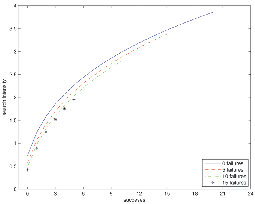
\includegraphics[width=\textwidth]{figures/figure2a.pdf}
        \caption{baseline}
        \label{fig:baseline_search_policy}
    \end{subfigure}
\par
\begin{subfigure}[b]{0.7\textwidth}
        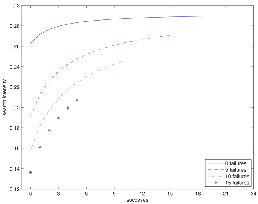
\includegraphics[width=\textwidth]{figures/figure2b.pdf}
        \caption{no network}
        \label{fig:no_network_search_policy}
    \end{subfigure}
\caption{\textbf{Search policy functions by match history}}
\label{fig:search_policy_outer}
\end{figure}

\bigskip

\subsection{Resticted versions of the model}

To explore identification of the learning effects and the reputation effects
in our model, we consider two alternative specifications. The first, which
we call the \textit{no-learning} model, treats firms as knowing their exact $%
\theta ^{f}$ draws, even before they acquire any experience in export
markets. This specification involves the same set of parameters, none of
which are constrained, so it isn't a nested version of the benchmark model.
Rather it replaces one characterization of beliefs with another. The second
alternative, which we call the \textit{no-network} model, is nested by the
benchmark model. It shuts down reputation effects by imposing $\gamma =0,$
but it retains the benchmark assumption that firms must learn their $\theta
^{f}$ draws through experience. Both alternative models are calibrated to the same statistics we use for our
benchmark model. The resulting parameter estimates and the associated fit
metrics are reported in Table \ref{tab:alt_est}. Below we discuss the ability of each to
fit the data.\bigskip

\begin{table}
    \centering
{\small 
\begin{tabular}{llrrr}
\multicolumn{5}{c}{\textbf{}} \\ \hline\hline
& \textit{Parameter} & \textit{benchmark} & \textit{no learning} & \textit{%
no network} \\ 
&  & \textbf{(}$\Lambda $\textbf{)} & \textbf{(}$\Lambda ^{NL}$\textbf{)} & 
\textbf{(}$\Lambda ^{NN}$\textbf{)} \\ \cline{2-5}
rate of exogenous separation & $\delta $ & 0.267 & 0.516 & 0.119 \\ 
domestic market size & $\Pi ^{h}$ & 11.344 & 12.670 & 10.884 \\ 
foreign market size & $\Pi ^{f}$ & 10.675 & 12.245 & 10.321 \\ 
fixed cost & $F$ & 7.957 & 10.238 & 8.539 \\ 
First $\theta $ distribution parameter & $\alpha $ & 0.716 & 0.512 & 1.807
\\ 
Second $\theta $ distribution parameter & $\beta $ & 3.161 & 0.351 & 0.963
\\ 
demand shock jump hazard & $\lambda _{y}$ & 0.532 & 0.713 & 1.581 \\ 
demand shock jump size & $\Delta ^{y}$ & 0.087 & 0.060 & 0.087 \\ 
shipment order arrival hazard & $\lambda _{b}$ & 8.836 & 10.028 & 10.347 \\ 
std. deviation, log firm type & $\sigma _{\varphi }$ & 0.650 & 1.268 & 1.355
\\ 
network effect parameter & $\gamma $ & 0.298 & 0.112 & 0 \\ 
\multicolumn{1}{c}{search cost function curvature parameter} & $\kappa _{1}$
& 0.087 & 0.0348 & 0.057 \\ 
search cost function scale parameter & $\kappa _{0}$ & 111.499 & 234.764 & 
175.953 \\ 
&  &  &  &  \\ 
fit metric & $D$ & 9.97 e+04 & 2.155 e+05 & 1.17 e+05 \\ 
fit metric, no weighting & $\widetilde{D}$ & 0.117 & 0.182 & 0.143 \\ \hline
\end{tabular}%
}
\caption{\textbf{Parameter Estimates for Alternative Models}}
\label{tab:alt_est}
\end{table}

\bigskip



\subsubsection{No learning}

Other things held fixed, the elimination of learning effects \ makes the
rapid turnover of novice exporters less likely, both by discouraging
inexperienced low-$\theta ^{f}$ firms from exploring foreign markets and by
eliminating learning-based exit. Shutting down learning effects also means
that high-$\theta ^{f}$ firms do not intensify their search efforts as they
receive positive feedback about their product appeal.

With these mechanisms inoperative, the no-learning model must use other
means to explain the rapid turnover of new exporters and the rapid expansion
of sales per surviving exporter as young cohorts mature. To accomplish the
former, lower productivity firms are induced to participate in export
markets by a rightward shift in the $\theta ^{f}$ distribution and higher
values for $\Pi ^{f}$ and $\lambda _{b}$, while match failure rates and
market exit rates are sustained by higher values for $F,$ $\delta ,$ and $%
\lambda _{y}$ (Table \ref{tab:alt_est}, column 3 versus column 2).\footnote{%
Recall that $E(\theta ^{f})=\alpha /(\alpha +\beta )$ and $var(\theta
^{j})=\alpha \beta /\left[ (\alpha +\beta +1)(\alpha +\beta )^{2}\right] .$}
\ To get sales per exporter growing with cohort age, the no-learning model
relies more heavily on selection effects. Low productivity firms are enticed
into the market by the bigger $\Pi ^{f}$ value and the higher average
popularity of their products. But these firms tend to end their matches as
soon as the fixed costs ($F$) come due, which--being relatively
large--ensures that the surviving exporters have substantially higher sales.
The relatively large value of $\lambda _{y}$ also helps to generate growth
in match sales conditioned on match survival, since buyers who draw negative
shocks tend to fail, while matches with positive shocks tend to survive.
Finally, the no-learning model facilitates new exporter growth by reducing
the convexity of the search cost function, $\kappa _{1}.$

While these parameter adjustments help the no-learning model qualitatively
match patterns of exporter turnover and growth, the model's overall fit
metric is much worse than that of the benchmark model (Table \ref%
{tab:alt_est}, lower panel)$.$ The reason is that the no-learning model
badly overstates the share of firms that export (Table \ref{tab:alt_fit} in
Appendix \ref{sec:restricted}), severely understates the persistence in
match-specific sales, given match continuation, overstates the relationship
between sales per client and number of clients, and fails to match the
Pareto shape of the cross exporter client distribution %.\newpage

\subsubsection{No network effect}

Network effects mean that sellers with a history of successful matches face
relatively low search costs, given search intensity. This allows firms with
popular products to build larger customer bases than the sharply convex
search cost function would have otherwise allowed, and thereby helps the
benchmark model match the Pareto distribution of clients across sellers.

To determine the importance of this feature of the model, we set $\gamma =0$
and re-estimated the remaining parameters, obtaining the no-network
estimates reported in Table \ref{tab:alt_est}. Without network effects, the the model moves part way toward matching the
Pareto shape by reducing the convexity of the search cost function, $\kappa
_{1}.$ But this is an imperfect fix because all exporters are equally
affected by $\kappa _{1}$, not just the larger ones. Accordingly, various
other adjustments occur, including a modest increase in $F$, a rightward
shift in the $\theta $ distribution, an increase in the variance of $\varphi
,$ and an increase in the jump hazard for buyer shocks, $\lambda _{y}.$
Interestingly, these adjustments are qualitatively similar to those that
occurred when we shut down learning effects. Here, however, market sizes $%
\Pi ^{f}$ and $\Pi ^{h}$ shrink a bit rather than expand.

Despite these adjustments, the no-network model does signficantly worse than
the benchmark model (Table \ref{tab:alt_est}, bottom panel). In particular,
the client distribution is far from Pareto, reflecting the model's inability
to explain the existance of very large exporters (Table \ref{tab:alt_fit} in
Appendix \ref{sec:restricted}). The no-network model also overstates the
fraction of firms that export and the average exports of surviving firms
after the first year. Finally, it makes the correlation between domestic and
foreign sales far too weak, and the log sales-per-client distribution far
too non-linear in the log of the number of clients.

The inability of the no-network model to generate a set of super-exporters
can be traced back to the search policy function this model delivers. Figure %
\ref{fig:no_network_search_policy} summarizes its properties. Note that
learning effects appear to be relatively important for the first several
clients, but unlike in figure \ref{fig:no_network_search_policy}, the policy
function quickly flattens out as successes accumulate. So, within the
general structure of our search and learning framework, sustained growth in
search intensity among relatively established exporters cannot be sustained
without network effects. Note also the very different scales between Figures %
\ref{fig:baseline_search_policy} and \ref{fig:no_network_search_policy},
indicating much lower search intensities when the network effect is not
present.

\subsection{Counterfactual experiments}

It remains to use our model to explore the export dynamics in a search and
learning world with network effects. These experiments will reveal the
extent to which learning and network effects create deviations from the
export path one would expect in a frictionless setting with the same
marketwide shocks and idiosyncratic processes for buyer and seller shocks.

We graph three experiments in Figures \ref{fig:search_dec_subplot}-\ref%
{fig:mac_bump_subplot} below. Each figure has separate panels decomposing
aggregate exports into number of exporters, mean per-client exports, and
mean number of clients. In Figure \ref{fig:search_dec_subplot}, we reduce
the scalar $\kappa _{0}$ in the search cost function by 20\% percent. In
Figure \ref{fig:cost_dec_subplot}, we decrease the fixed cost of maintaining
a client relationship $F$ by 20\%, and in Figure \ref{fig:mac_bump_subplot},
we reduce the size of foreign market jumps $\Delta {x_{f}}$ by 20\%
percent. For all experiments, the shock takes place in 2002 and is
unanticipated and permanent. The red line represents the time path that
would have been observed in the absence of the shock, and the dashed blue
line reflects the time path induced by the shock. We use the same draws for
all stochastic processes, with and without the parameter change, so these
changes are the only reason that the blue line differs from the red line
after 2002. In all exercises, we take the market-wide demand shifters $x_{f}$
and $x_{h}$ from the data.

While the shock takes place in 2002, decreasing the cost of search has no
noticeable net effect on exports until 2003. The slow reaction of firms to
shocks is a theme in all of our counterfactuals. The decrease in search
costs appears to mainly encourage inexperienced firms to search harder.
Since exporters start small, and this is reflected in a decrease in mean
sales per client, the initial effect on aggregate exports is small. Over
time, however, a successful exporter will ramp up her search behavior, so
that aggregate exports ultimately grow relative to the baseline.

Exporters also react slowly to the fixed cost reduction in Figure \ref%
{fig:cost_dec_subplot}, and different margins react with different speeds.
While the number of active exporters does most of its jumping in 2002, the mean
number of clients rises more gradually as it takes all exporters time to
acquire the new equilibrium collection of clients.

Somewhat surprisingly, decreasing fixed cost does not cause mean sales per
client to drop. Mean sales are affected by two margins. For a particular
firm, mean sales per client will decrease as poor clients that would have
been let go are allowed to stick around. On the other hand, lowering fixed
costs also encourages highly productive firms to search harder. Since the
typical match relationship at one of the best firms is highly lucrative, a
new match can cause economy-wide mean sales per client to rise. That mean
sales per client rise after decreasing fixed costs suggests that productive
firms gain more new clients than unproductive firms.

Both a reduction in search costs and a reduction in fixed costs per shipment
could be potentially interpreted as policy experiments. For instance,
Proexport, the Colombian export promotion agency, has several programs aimed
at helping firms find foreign clients. These range from publishing lists of
potential buyers in their website to firm-specific studies and trips
organized by Proexport (some of which the firm itself pays for). The
introduction of this type of programs, or subsidized prices for them could
lead to reduced search costs. As for the fixed cost per shipment,
regulations may also affect these costs. The World Bank, for instance,
estimates that in 2005 the fees associated with procedures to export goods
amounted to \$1,745 per one-container shipment.

Figure \ref{fig:cost_dec_subplot} shows the results of the experiment where
the foreign market size suddenly increases by 20 percent. All matches become
more lucrative. This mechanical rise in sales explains the sudden increase
in exports and mean sales per client immediately after the shock. The
gradual reaction of exports can be seen in the mean number of clients per
exporter, which takes almost a decade to fully react to the shock.

\pagebreak

\begin{figure}[tbp]
\centering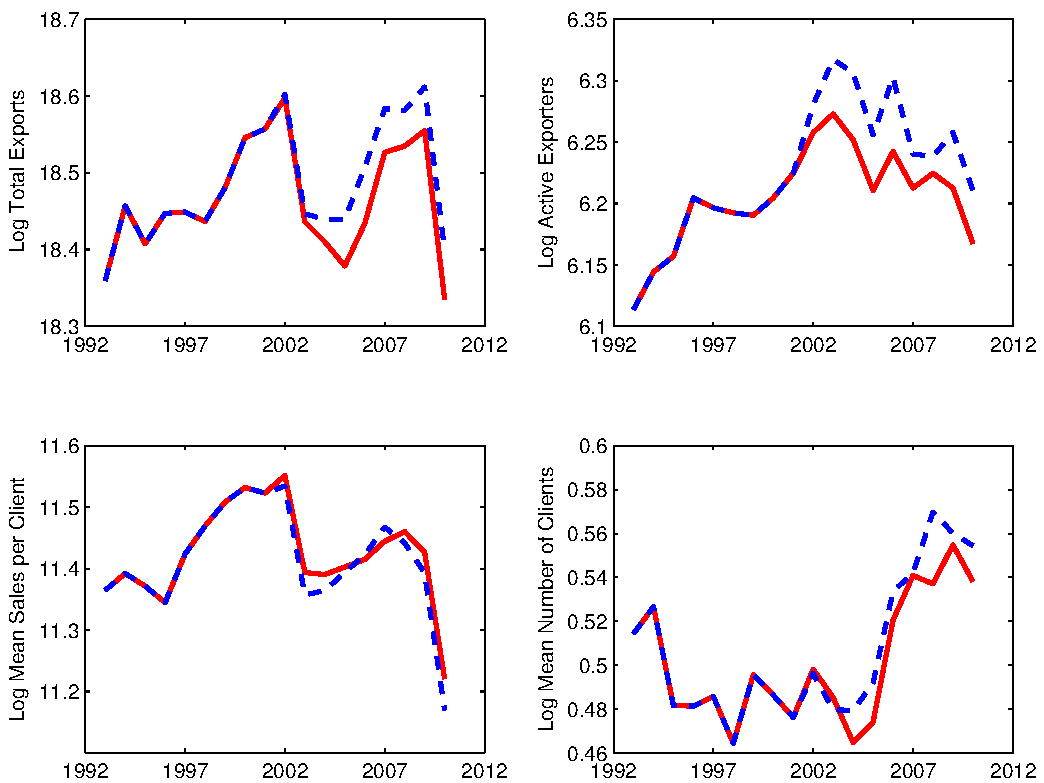
\includegraphics[width=\textwidth]{figures/figure3-eps-converted-to.pdf}
\caption{\textbf{Time Series Effects of Search Cost Reduction}}
\label{fig:search_dec_subplot}
\end{figure}
\newpage

\begin{figure}[tbp]
\centering
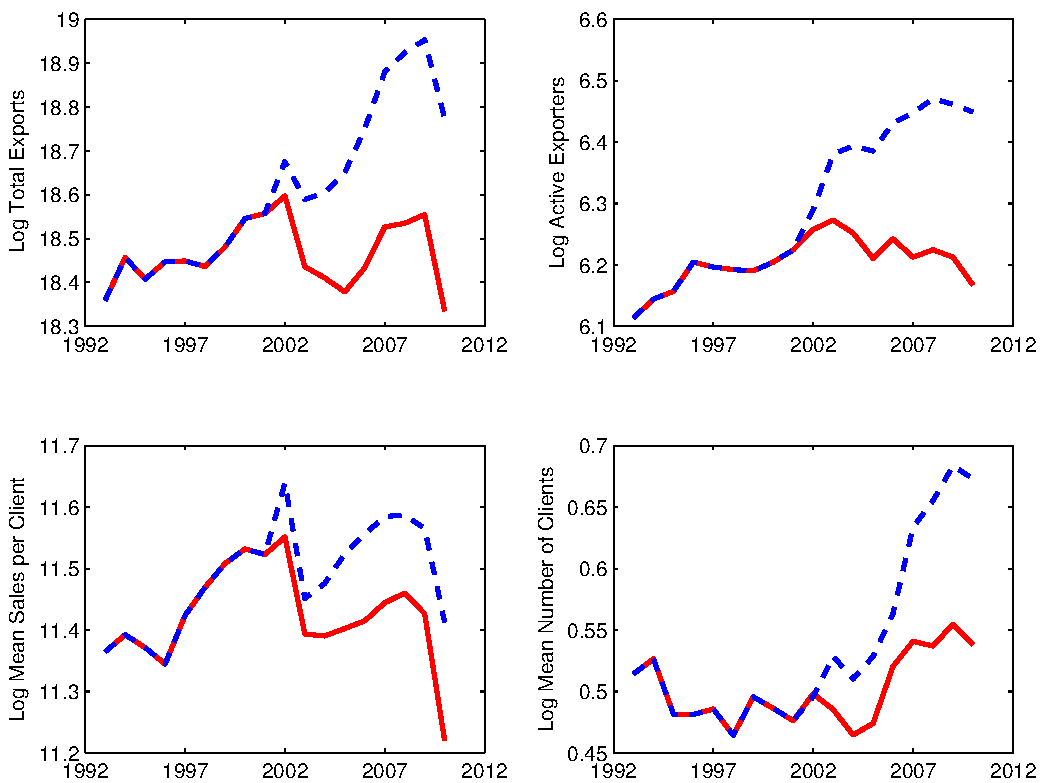
\includegraphics[width=\textwidth]{figures/figure4-eps-converted-to.pdf}
\caption{\textbf{Time Series Effects of Fixed Cost Reduction}}
\label{fig:cost_dec_subplot}
\end{figure}
\newpage

\begin{figure}[tbp]
\centering
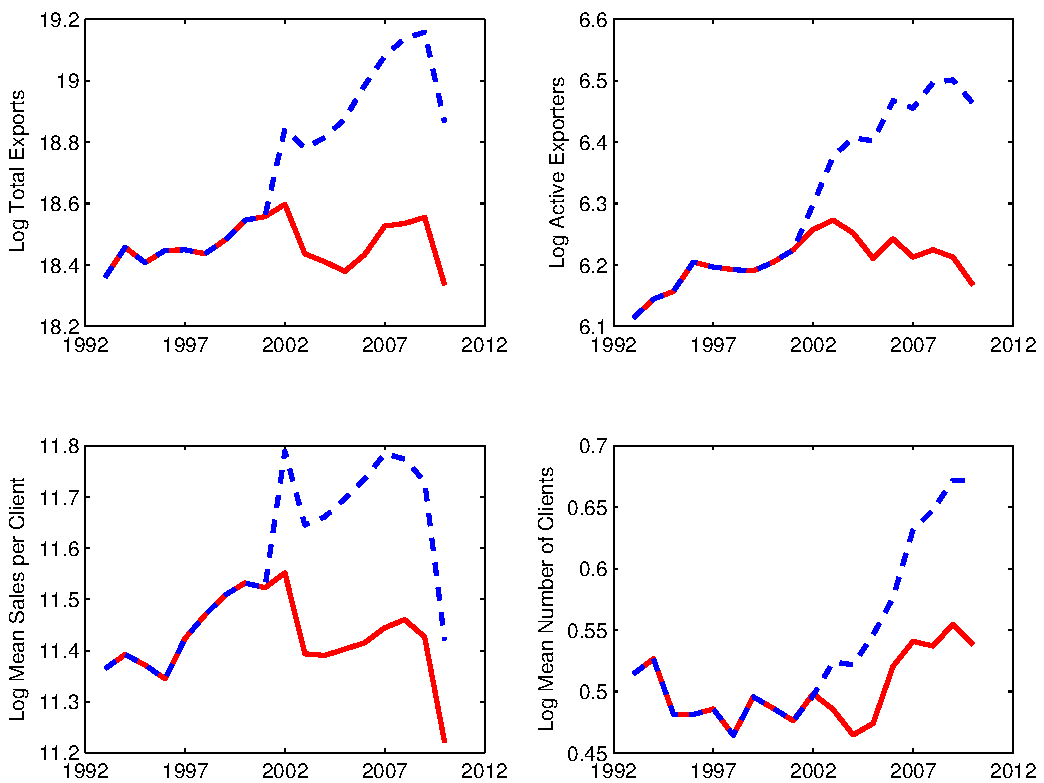
\includegraphics[width=\textwidth]{figures/figure5-eps-converted-to.pdf}
\caption{\textbf{Time Series Effects of Positive Market-wide Shock}}
\label{fig:mac_bump_subplot}
\end{figure}

\pagebreak % \begin{center}
% \textbf{Figure 4: Time Series Effects of Search Cost Reduction}\FRAME{ftbpF}{%
% 5.3298in}{4.1364in}{0pt}{}{}{search_dec_subplot.eps}{\special{language
% "Scientific Word";type "GRAPHIC";maintain-aspect-ratio TRUE;display
% "USEDEF";valid_file "F";width 5.3298in;height 4.1364in;depth
% 0pt;original-width 6.89in;original-height 5.3411in;cropleft "0";croptop
% "1";cropright "1";cropbottom "0";filename
% './search_dec_subplot.eps';file-properties "XNPEU";}}\pagebreak
%
% \textbf{Figure 5: Time series effects of Fixed Cost Reduction}
% 
% \FRAME{ftbpF}{5.4803in}{4.3076in}{0pt}{}{}{cost_dec_subplot.eps}{\special%
% {language "Scientific Word";type "GRAPHIC";maintain-aspect-ratio
% TRUE;display "USEDEF";valid_file "F";width 5.4803in;height 4.3076in;depth
% 0pt;original-width 6.8044in;original-height 5.3411in;cropleft "0";croptop
% "1";cropright "1";cropbottom "0";filename
% './cost_dec_subplot.eps';file-properties "XNPEU";}}\pagebreak
% 
% \begin{center}
% \textbf{Figure 6: Time Series Effects of Positive Market-wide Shock}
% \end{center}
% 
% \FRAME{ftbpF}{5.5011in}{4.3223in}{0pt}{}{}{mac_bump_subplot.eps}{\special%
% {language "Scientific Word";type "GRAPHIC";maintain-aspect-ratio
% TRUE;display "USEDEF";valid_file "F";width 5.5011in;height 4.3223in;depth
% 0pt;original-width 6.8044in;original-height 5.3411in;cropleft "0";croptop
% "1";cropright "1";cropbottom "0";filename
% './mac_bump_subplot.eps';file-properties "XNPEU";}}

% \pagebreak

\section{Summary}

Customs records reveal tremendous turnover among Colombian manufacturers who
export to the U.S.. In a typical year, 48 percent of these exporters are new
to the U.S. market, and 81 percent of these new exporters will be gone two
years hence. New exporters ship small quantities, so despite their numbers
they account for only 12 percent of total Colombian exports in value terms.
But each new cohort of Colombian exporters contains a small
number of firms that survive and rapidly expand, growing many times faster
than aggregate Colombian exports. They do so by adding U.S. clients to their
customer base at a rapid rate.

After documenting these patterns, we develop a continuous time model that
explains them. Firms wishing to export must engage in costly search to
identify potential buyers abroad. The buyers they encounter either reject
their products or form finite-lived business relationships with them. Buyer
who form business relationships with exporters send them favorable signals
about the appeal of their products, and in doing so, encourage them to
search more intensively for additional buyers. Successful business
relationships also reduce search costs by improving sellers' visibility
(network effects). Finally, sellers' search intensities depend upon their
permanent idiosyncratic characteristics and marketwide conditions.

Fit using the method of simulated moments, the model replicates the patterns
in customs records described above and allows us quantify several types of
trade costs, including the search costs of identifying potential clients and
the costs of maintaining business relationships with existing clients. It
also allows us to estimate the network effect of previous exporting
successes on the costs of meeting new clients, and to characterize the
cumulative effects of learning on firms'search intensities. Both the
learning effect and the network effect prove to be quantitatively important.
Finally, our model provides a lens through which to view the seemingly
unpredictable responses of export flows to exchange rate fluctuations.

\begin{center}
\ \pagebreak

{\Large \textbf{References}}
\end{center}

\begin{description}
\item Albornoz, Facundo, Hector Calvo Pardo, Gregory Corcos, and Emanuel
Ornelas (2012) "Sequential Exporting," \textit{Journal of International
Economics} 88: 17-31.

\item Alessandria, George and Horag Choi (2007) "Do Sunk Costs of Exporting
Matter for Net Export Dynamics?" \textit{Quarterly Journal of Economics},
pp. 289-336.

\item Alessandria,\ George, Joseph Kaboski and Virgiliu Midrigan (2010)
"Inventories, Lumpy Trade, and Large Devaluations," \textit{American
Economic Review}, 100 (5) pp. 2304-39.

\item Arkolakis, Konstantinos (2009) \textquotedblleft A Unified Theory of
Firm Selection and Growth,\textquotedblright\ Yale University, Department of
Economics, Working Paper.

\item Arkolakis, Konstantinos (2010) \textquotedblleft Market Access Costs
and the New Consumers Margin in International Trade,\textquotedblright\ 
\textit{Journal of Political Economy}, 118(6), pp. 1151-1199.

\item Baldwin, Richard. E. and Paul Krugman (1989): \textquotedblleft
Persistent Trade Effects of Large Exchange Rate Changes.\textquotedblright\ 
\textit{Quarterly Journal of Economics}, 104, pp. 635-654.

\item Bernard, Andrew and J. Bradford Jensen (1999) \textquotedblleft
Exceptional Exporter Performance: Cause, Effect, or Both?\textquotedblright\ 
\textit{Journal of International Economics} , 47, pp. 1-25.

\item Bernard, Andrew, J. Bradford Jensen, Samuel Kortum and\ Jonathan Eaton
(2003) \textquotedblleft Plants and Productivity in International
Trade,\textquotedblright\ \textit{American Economic Review }93(4), pp.
1268-1290

\item Bernard, Andrew, J. Bradford Jensen, J. Stephen J. Reading, and Peter
K. Schott (2007) \textquotedblleft Firms in International
Trade,\textquotedblright\ \textit{Journal of Economic Perspectives}.

\item Besedes, Tibor (2007). \textquotedblleft A Search Cost Perspective on
Formation and Duration of Trade,\textquotedblright\ Working Paper,
Department of Economics, Georgia Tech University.

\item Blum, Bernardo S., Sebastian Claro, and Ignatius Horstmann (2009).
\textquotedblleft Intermediation and the Nature of Trade Costs: Theory and
Evidence.\textquotedblright\ Working Paper, The University of Toronto.

\item Brooks, Eileen (2006) \textquotedblleft Why don't firms export more?
Product Quality and Colombian Plants\textquotedblright\ \textit{Journal of
Development Economics,} 80: 160-178.

\item Chaney, Thomas (2011) \textquotedblleft The Network Structure of
International Trade,\textquotedblright\ University of Chicago.

\item Clerides, Sofronis, Saul Lach and\ James Tybout (1998)
\textquotedblleft Is Learning-by-Exporting Important? Micro-dynamic Evidence
from Colombia, Mexico and Morocco,\textquotedblright\ \textit{Quarterly
Journal of Economics}, pp. 903-947.

\item Das, Mita, Mark Roberts and James Tybout (2007) \textquotedblleft
Market Entry Costs, Producer Heterogeneity and Export
Dynamics,\textquotedblright\ \textit{Econometrica }75(3), pp. 837-874.

\item Dom\'{\i}nguez, Juan Camilo, Jonathan Eaton, Marcela Eslava, and James
Tybout. (2010) "Search and Learning in Export Markets: Case Studies for
Colombia." Pennsylvania State University, Working Paper.

\item Drozd, Lukasz A. and Jaromir B. Nosal (2008) \textquotedblleft
Understanding International Prices: Customers as Capital,\textquotedblright\
Working Paper, The University of Wisconsin.

\item Dixit, Avinish (1989), \textquotedblleft Hysteresis, Import
Penetration, and Exchange Rate Pass-Through,\textquotedblright\ \textit{%
Quarterly Journal of Economics}, Vol. 104, No. 2 (May), pp. 205-228.

\item Eaton, Jonathan, Samuel Kortum, and Francis Kramarz (2004)
\textquotedblleft Dissecting Trade: Firms, Industries, and Export
Destinations,\textquotedblright\ \textit{American Economic Review Papers and
Proceedings,} 94: 150-154.

\item Eaton, Jonathan, Samuel Kortum, and Francis Kramarz (2011)
\textquotedblleft An Anatomy of International Trade: Evidence from French
Firms,\textquotedblright\ \textit{Econometrica} 79(5), pp. 1453-1498.

\item Eaton, Jonathan, Marcela Eslava, Maurice Kugler and James Tybout
(2008). \textquotedblleft Export Dynamics in Colombia: Firm-Level
Evidence,\textquotedblright\ in Elhanan Helpman, Dalia Marin and Thierry
Verdier, eds., T\textit{he Organization of Firms in a Global Economy},
Cambridge, MA: Harvard U. Press.

\item Eslava, Marcela, John Haltiwanger, Adriana Kugler, and Maurice Kugler
(2004) \textquotedblleft The Effects of Structural Reforms on Productivity
and Profitability Enhancing Reallocation: Evidence from
Colombia,\textquotedblright\ \textit{Journal of Development Economics,} 75:
333-371.

\item Gouri\'{e}roux and Monfort, 1996. \textit{Simulation-Based Econometric
Methods}. New York: Oxford U. Press.

\item Irarrazabal, Alfonso A. and Luca David Opromolla (2006)
\textquotedblleft Hysteresis in Export Markets,\textquotedblright\ New York
University, Working Paper.

\item Jackson, Matthew and Brian Rogers (2007) \textquotedblleft Meeting
Strangers and Friends of Friends: How Random are Social
Networks?\textquotedblright\ \emph{American Economic Review,} 97: 890-915.

\item Jovanovic, Boyan (1982) \textquotedblleft Selection and the Evolution
of Industry,\textquotedblright\ \textit{Econometrica,} 50: 649-670.

\item Kugler, Maurice (2006) \textquotedblleft Spillovers from foreign
direct investment: within or between industries?\textquotedblright\ \textit{%
Journal of Development Economics, }80(2): 444-477.

\item Luttmer, Erzo (2007) \textquotedblleft Selection, Growth, and the Size
Distribution of Firms,\textquotedblright\ \textit{Quarterly Journal of
Economics,} 122: 1103-1144.

\item Melitz, Marc (2003) \textquotedblleft The Impact of Trade on
Intra-Industry Reallocations and Aggregate Industry
Productivity,\textquotedblright\ \textit{Econometrica }71, 1695-1725.

\item Rauch, James and Joel Watson (2003) \textquotedblleft Starting Small
in an Unfamiliar Environment,\textquotedblright\ \textit{International
Journal of Industrial Organization} 21: 1021-1042.

\item Roberts, Mark and James Tybout (1997a) \textquotedblleft The Decision
to Export in Colombia: An Empirical Model of Entry with Sunk
Costs,\textquotedblright\ \textit{American Economic Review} 87(4), pp.
545-563.

\item Roberts, Mark and James Tybout (1997b) \textit{What Makes Exports Boom}%
? Directions in Development Monograph Series, The World Bank, Washington, DC.

\item Ruhl, Kim and Jonathan Willis (2008) \textquotedblleft New Exporter
Dynamics,\textquotedblright\ New York University, Working Paper.

\item Shimer, Robert (2005) "The Cyclical Behavior of Equilibrium
Unemployment and Vacancies," \textit{The American Economic Review}, 95(1),
pp. 25-49.

\item Tauchen, George (1986) \textquotedblleft Finite State Markov-Chain
Approximation to Univariate and Vector Autoregressions,\textquotedblright\ 
\textit{Economics Letters,} 20.2. 177-181.\pagebreak
\end{description}

%\appendix
\section{Data Checks}
\label{sec:data_check}

To investigate the quality of the exporter id (manuf\_id) in the U.S. import
records, we ran a series of robustness checks. The Colombian and U.S. data
overlap for the years 2000-2008 and both contain measures of the value of
exports as well as the number of exporting firms. If the manuf\_id variable
is error-prone and noisy, we would expect the U.S. data to over-report the
number of Colombian firms exporting to the U.S. That is, each time a customs
broker wrongly enters the data in the field, a new firm would be created.
Table \ref{tab:ap_dat_comp} below summarizes the total value of exports to the U.S. and the
number of Colombian firms, by year, for each data set.

\begin{table}
    \centering
{\small 
\begin{tabular}{l}
%\begin{tabular}{rrrrrrr}
\begin{tabular}{rrrrlrr} \hline \hline 

& \multicolumn{2}{r}{\textbf{Colombia}} & \multicolumn{2}{r}{\textbf{United
States}} & \multicolumn{2}{r}{\textbf{\% difference}} \\ \cline{2-7}
Year & \# exporters & value & \# exporters & value & \# exporters & value \\ 
\hline
2000 & 1775 & 1038 & 2721 & 1140 & 53\% & 10\% \\ 
2001 & 2026 & 995 & 2744 & 1019 & 35\% & 2\% \\ 
2002 & 2230 & 870 & 2986 & 855 & 34\% & -2\% \\ 
2003 & 2800 & 1113 & 3579 & 1119 & 28\% & 1\% \\ 
2004 & 3035 & 1379 & 4002 & 1415 & 32\% & 3\% \\ 
2005 & 2861 & 1554 & 4288 & 1438 & 50\% & -7\% \\ 
2006 & 2689 & 1665 & 4361 & 1552 & 62\% & -7\% \\ 
2007 & 2420 & 1540 & 4175 & 1496 & 73\% & -3\% \\ 
2008 & 2161 & 1570 & 3758 & 1474 & 74\% & -6\% \\ \hline
\end{tabular}%
\end{tabular}%
}
\caption{\textbf{Colombian versus U.S. Customs Records}}
\label{tab:ap_dat_comp}
\end{table}

The datasets align much more closely on value than they do on firm counts.
The difference in value is never more than 10\% while the firm count
difference ranges from 18\% to 74\%. The differences are stable over time.

To look more closely at the cause of the difference in firm counts, we
compared the number of firms across sources by HS2 categories. The counts in
the LFTTD were higher than the Colombian data in only 28 of the 82 codes and
by far the biggest differences are in HS codes 61 and 62: textiles. In these
two product classes the U.S. data identifies 4025 more firms than the
Colombian data. If we remove these two sectors from the list, the difference
in firm counts flips and the Colombian data contain 1001 more firms than the
LFTTD.

Interestingly, Title 19 of U.S. code specifically requires that the
manuf\_id variable for textile products represent the manufacturer of the
textile products, not an intermediary. That is, for this sector in
particular the manufacturer, not an intermediary must be reported on the CBP
7501 form. By contrast, prior work by several authors of this paper has
shown (Marcela's 8/9/13 e-mail referenced this) that the Colombian data
reports the exporter, which may or may not be the manufacturer. Given that
revious research (Tybout, 2000 JEL) has shown that developing countries tend
to have a disproportionately large share of small manufacturing firms, it is
reasonable to assume that a large part of the reason why the U.S. data
report so many more firms in the textile sector is that due to
administrative reasons the U.S. data count many small manufacturers and the
Colombian data are, in many cases, reporting aggregators and intermediaries.

As a final check of the integrity of the manuf\_id variable - and the
robustness of our main results - we experimented with a \textquotedblleft
fuzzy\textquotedblright\ version of the manuf\_id variable that did not
contain any street numbers in the string (a likely source of input errors).
The effect of this is to reduce the number of Colombian firms in the data,
an approximation of fixing any extraneous noise from data entry errors. Next
we re-ran Table \ref{tab:sep_rates} with the fuzzy data and compared the results to the
original version.

One of the key findings from Table \ref{tab:sep_rates} is the high match separation rates
ranging from about 40\% to 66\%. Using the fuzzy version did not reduce the
separation rates substantially and left the patterns intact. The fuzzy
separation rates ranged from 26\% to 62\%, a drop of 6\% on average. It does
not appear that our results are sensitive to a modest reduction in data
entry errors.
 
\section{Moments for Restricted Models}
\label{sec:restricted}
\begin{small}
\begin{longtable}{l|rrrr}
    %\caption{}
\caption[Restricted versus Full Model Fit]{Restricted versus Full Model Fit} \label{tab:alt_fit} \\ \hline \hline
    & \emph{data} & \emph{benchmark} & \emph{no learning} & \emph{no network} \\ 
& $\widehat{M}$ & $M_{s}(\Lambda )$ & $M_{s}(\Lambda ^{NL})$ & $M_{s}(\Lambda ^{NN})$ \\ \cline{2-5}
\textbf{Share of firms exporting} &  &  &  &  \\ 
$\widehat{E}(1_{X_{jt}^{f}>0})$ & 0.299 & 0.351 & 0.585 & 0.451 \\ 
&  &  &  &  \\ 
\textbf{Log foreign sales on} &  &  &  &  \\ 
\textbf{log domestic sales} &  &  &  &  \\ 
$\widehat{\beta }_{1}^{hf}$ & 0.727 & 0.515 & 0.923 & 0.575 \\ 
$s\widehat{e}(\epsilon ^{hf})$ & 2.167 & 1.424 & 0.843 & 1.146 \\ 
\multicolumn{1}{r}{} &  &  &  &  \\ 
\textbf{log dom. sales autoreg.} &  &  &  &  \\ 
$\widehat{\beta }_{1}^{h}$ & 0.976 & 0.896 & 0.969 & 0.898 \\ 
$s\widehat{e}(\epsilon ^{h})$ & 0.462 & 0.683 & 0.661 & 0.570 \\ 
&  &  &  &  \\ 
\textbf{exporter exit hazards} &  &  &  &  \\ 
$\widehat{E}[1_{X_{jt}^{f}=0}|A_{jt-1}^{c}=0]$ & 0.709 & 0.748 & 0.773 & 
0.877 \\ 
$\widehat{E}[1_{X_{jt}^{f}=0}|A_{jt-1}^{c}=1]$ & 0.383 & 0.099 & 0.099 & 
0.188 \\ 
$\widehat{E}[1_{X_{jt}^{f}=0}|A_{jt-1}^{c}=2]$ & 0.300 & 0.121 & 0.032 & 
0.012 \\ 
$\widehat{E}[1_{X_{jt}^{f}=0}|A_{jt-1}^{c}=3]$ & 0.263 & 0.055 & 0.056 & 
0.198 \\ 
$\widehat{E}[1_{X_{jt}^{f}=0}|A_{jt-1}^{c}=4]$ & 0.293 & 0.100 & 0.098 & 
0.185 \\ 
\textbf{log sales per exporter} &  &  &  &  \\ 
\textbf{by cohort age } &  &  &  &  \\ 
$\widehat{E}(\ln X_{jt}^{f}|A_{jt}^{c}=0)$ & 8.960 & 9.306 & 9.608 & 8.541
\\ 
$\widehat{E}(\ln X_{jt}^{f}|A_{jt}^{c}=1)$ & 10.018 & 10.806 & 10.615 & 
11.331 \\ 
$\widehat{E}(\ln X_{jt}^{f}|A_{jt}^{c}=2)$ & 10.231 & 10.755 & 10.431 & 
11.037 \\ 
$\widehat{E}(\ln X_{jt}^{f}|A_{jt}^{c}=3)$ & 10.369 & 10.679 & 10.426 & 
10.845 \\ 
$\widehat{E}(\ln X_{jt}^{f}|A_{jt}^{c}\geq 4)$ & 10.473 & 10.669 & 10.332 & 
11.145 \\
\textbf{Log match sale autoregression} &  &  &  &  \\ 
$\widehat{\beta }_{1}^{f}$ & 0.811 & 0.613 & 0.105 & 0.268 \\ 
$\beta _{\mbox{1st
year}}^{f}$ & 0.233 & 0.370 & 0.056 & 0.087 \\ 
$s\widehat{e}(\epsilon ^{f})$ & 1.124 & 0.503 & 0.287 & 0.425 \\ 
&  &  &  &  \\ 
\textbf{Match death hazards} &  &  &  &  \\ 
$\widehat{E}[1_{X_{ijt}^{f}=0}|X_{ijt-1}^{f}>0,A_{ijt-1}^{m}=0]$ & 0.694 & 
0.857 & 0.943 & 0.879 \\ 
$\widehat{E}[1_{X_{ijt}^{f}=0}|X_{ijt-1}^{f}>0,A_{ijt-1}^{m}=1]$ & 0.515 & 
0.329 & 0.452 & 0.337 \\ 
$\widehat{E}[1_{X_{ijt}^{f}=0}|X_{ijt-1}^{f}>0,A_{ijt-1}^{m}=2]$ & 0.450 & 
0.304 & 0.426 & 0.286 \\ 
$\widehat{E}[1_{X_{ijt}^{f}=0}|X_{ijt-1}^{f}>0,A_{ijt-1}^{m}=3]$ & 0.424 & 
0.281 & 0.434 & 0.332 \\ 
$\widehat{E}[1_{X_{ijt}^{f}=0}|X_{ijt-1}^{f}>0,A_{ijt-1}^{m}=4]$ & 0.389 & 
0.305 & 0.398 & 0.226 \\ 
\multicolumn{1}{r}{} &  &  &  &  \\ 
\textbf{Match death prob regression} &  &  &  &  \\ 
$\widehat{\beta }_{0}^{d}$ & 1.174 & 1.640 & 1.843 & 2.087 \\ 
$\widehat{\beta }_{\mbox{1st year}}^{d}$ & 0.166 & 0.203 & 0.031 & 0.055 \\ 
$\widehat{\beta }_{\mbox{lsales}}^{d}$ & -0.070 & -0.100 & -0.092 & -0.140
\\ 
$s\widehat{e}(\epsilon ^{d})$ & 0.453 & 0.395 & 0.266 & 0.343 \\ 
\multicolumn{1}{r}{} &  &  &  &  \\ 
\textbf{Match shipments per year} &  &  &  &  \\ 
$\widehat{E}\left( n^{s}\right) $ & 4.824 & 3.770 & 2.064 & 4.525 \\
\textbf{Transition probabilities, } &  &  &  &  \\ 
\textbf{No. clients (}$n^{c}$\textbf{)} &  &  &  &  \\ 
$\widehat{P}[n_{jt+1}^{c}=0|n_{jt}^{c}=1]$ & 0.618 & 0.534 & 0.677 & 0.643
\\ 
$\widehat{P}[n_{jt+1}^{c}=1|n_{jt}^{c}=1]$ & 0.321 & 0.358 & 0.255 & 0.307
\\ 
$\widehat{P}[n_{jt+1}^{c}=2|n_{jt}^{c}=1]$ & 0.048 & 0.082 & 0.056 & 0.045
\\ 
$\widehat{P}[n_{jt+1}^{c}\geq 3|n_{jt}^{c}=1]$ & 0.013 & 0.024 & 0.010 & 
0.004 \\ 
$\widehat{P}[n_{jt+1}^{c}=0|n_{jt}^{c}=2]$ & 0.271 & 0.260 & 0.456 & 0.165
\\ 
$\widehat{P}[n_{jt+1}^{c}=1|n_{jt}^{c}=2]$ & 0.375 & 0.321 & 0.291 & 0.306
\\ 
$\widehat{P}[n_{jt+1}^{c}=2|n_{jt}^{c}=2]$ & 0.241 & 0.281 & 0.166 & 0.427
\\ 
$\widehat{P}[n_{jt+1}^{c}\geq 3|n_{jt}^{c}=2]$ & 0.113 & 0.135 & 0.086 & 
0.100 \\ 
&  &  &  &  \\ 
\textbf{Log sales per client on} &  &  &  &  \\ 
\textbf{client no. regression} &  &  &  &  \\ 
$\widehat{\beta }_{1}^{m}$ & 2.677 & 0.842 & 0.944 & 3.887 \\ 
$\widehat{\beta }_{2}^{m}$ & -0.143 & 0.042 & 1.049 & -1.451 \\ 
$s\widehat{e}(\epsilon ^{m})$ & 2.180 & 1.622 & 1.893 & 2.067 \\ 
&  &  &  &  \\ 
\textbf{Client number inverse} &  &  &  &  \\ 
\textbf{CDF regression} &  &  &  &  \\ 
$\widehat{\beta _{1}}^{c}$ & -1.667 & -1.587 & -1.395 & -1.655 \\ 
$\widehat{\beta _{2}}^{c}$ & -0.097 & -0.280 & -1.184 & -1.420 \\ 
$s\widehat{e}(\epsilon ^{n^{c}})$ & 0.066 & 0.128 & 0.062 & 0.069 \\ \hline
\end{longtable}
\end{small}
